\chapter{Applications}
\label{chap:numres}
After developing the tools for obtaining information about bath
related observables in \cref{chap:flow} and the means for their
verification in \cref{chap:analytsol}, we are now in a position to
apply those results.

The roadmap is the following. Using \cref{chap:analytsol} we will
verify the results of \cref{chap:flow} in \cref{sec:hopsvsanalyt}.  A
striking phenomenon will be noticed and explained in a brief detour
\cref{sec:pure_deph}.

In the generic case where no analytic solution we nevertheless are
able to obtain consistent results as is demonstrated in
\cref{sec:prec_sim}.

These results will strengthen the confidence in
the method so that we can turn to more complicated applications.
First a brief overview of interesting features of quantum
thermodynamics is given in \cref{sec:basic_thermo}. Subsequently we
will turn to two applications to demonstrate these features in
\cref{sec:singlemod,sec:otto}.

An overview and explanation of the codes used in this chapter can be found
in \cref{sec:code}.

\section{Some Remarks on the Methods}
\label{sec:meth}
Before we begin with the applications in earnest, let us review some
technical details.

The figures presented may feature error funnels whose origin is,
unless otherwise stated, estimated from the empirical standard
deviation of the calculated quantities due to the finite sample
size. As the quantities that are being calculated using HOPS are
essentially Monte Carlo integrals, those statistical errors scale as
\(1/\sqrt{N}\) with the sample size \(N\) and therefore controllable
besides being simple to estimate. Note however, that a certain number
of samples is required to estimate the standard deviation of a single
trajectory correctly.

To tell whether some vector quantities\footnote{For example a time
  series.} \(X_1, X_2\) obtained with HOPS or otherwise are compatible
with each other or an analytical result, we consider the quantity
\(Δ=X_1 - X_2\). Assuming all numerical errors are negligible, we
demand that \(\abs{Δ} \leq σ_Δ\) for at least \(68\%\) of the entries
of the \(X_i\), where \(σ_Δ\) is the standard deviation due to the
stochastic sampling. This percentage is often displayed in legends as
a number in parentheses.

For the estimation of mean and standard deviation from trajectory
data, Welford's online algorithm is employed to avoid catastrophic
numerical cancellation~\cite{Welford1962Aug,Knuth1997}.

In all simulations discussed an Ohmic spectral density
\begin{equation}
  \label{eq:ohmic_sd}
  J(ω)=η ω \eu^{-\frac{ω}{ω_{c}}}\quad (ω>0)
\end{equation}
is used unless otherwise. This spectral density models an environment
with a physical energy spectrum that is bounded from below and allows
the application of the finite temperature method described
in~\cite{RichardDiss} and \cref{sec:lin_finite}. Also, \(J(0) = 0\)
ensures that there is a unique zero temperature state of the
bath. In~\cite{Kolar2012Aug} it is argued (under weak coupling
assumptions), that \(J(ω)\approx ω^γ\) with \(γ<1\) could lead to a
violation of the third law.  Physically, a scaling of the spectral
density \(\propto ω\) is connected to acoustic
phonons~\cite{Kolar2012Aug}.

In \cref{eq:ohmic_sd} \(η\) is a scaling
constant and \(ω_c\) (the cutoff frequency) regulates the decay of the
spectral density. The corresponding bath correlation function (BCF)
is
\begin{equation}
  \label{eq:ohmic_bcf}
  α(τ) = \frac{1}{π} ∫\dd{ω} J(ω) \eu^{-\iu ωτ} =
  \frac{η}{π}\qty(\frac{ω_c}{1+\iu ω_c τ})^2.
\end{equation}
We see that higher cutoff frequencies correspond to a faster decay of
the bath correlation function. This parameter provides control over
the ``Markovianity'' of the bath.

It may be remarked, that~\cref{eq:ohmic_bcf} does not correspond to a
simple sum of exponentials. As such it exercises the HOPS method and
serves as a model for a general bath correlation function. For use
with HOPS, a sum of exponentials must be fitted to the BCF. In
\cref{sec:hopsvsanalyt} we will see, that this is indeed a valid
strategy.

Throughout this chapter, we will only apply the nonlinear
method~\cite{Hartmann2017Dec} described in \cref{sec:nmqsd_basics}
(see also \cref{sec:nonlin_flow}).

\section{Comparison with an Analytical Solution}
\label{sec:hopsvsanalyt}
In \cref{chap:analytsol} and specifically \cref{sec:oneosc,sec:twoosc}
an analytical solution for a quantum Brownian motion like model was
derived. Using this solution, we are able to verify the results of
\cref{chap:flow} and benchmark the HOPS method. It will be shown, that
HOPS can indeed reproduce the \emph{exact} open system dynamics of the
bath energy flow.

\subsection{A Harmonic Oscillator coupled to a single Bath}
\label{sec:oneosccomp}
We begin with the simplest possible model of a single zero temperature
bath.  For the simulations with HOPS the model
\cref{eq:one_ho_hamiltonian} was made dimensionless by choosing
\(Ω=1\). Simulations were run for both for zero temperature and a
finite temperature with varying bath correlation functions.

\begin{figure}[t]
  \centering
  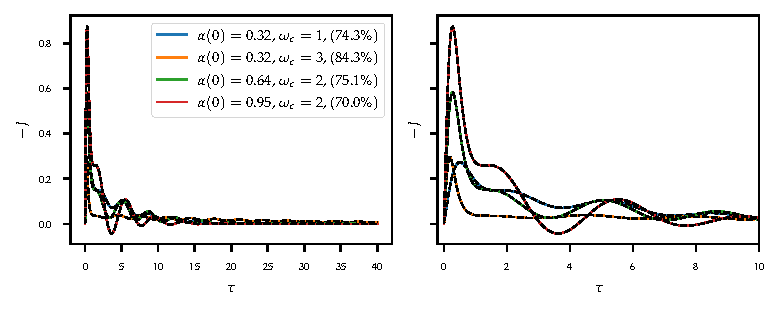
\includegraphics{figs/analytic_comp/flow_comp_zero.pdf}
  \caption{\label{fig:comp_zero_t} The bath energy flow \(-J\) for
    different parameters of the ohmic bath correlation function
    \cref{eq:ohmic_bcf}. The solid lines have been obtained with HOPS
    and the dashed lines using the analytic solution. A good agreement
    is evident visually and corroborated by the consistency values in
    the legend (see \cref{sec:meth} for an explanation).  The
    simulation with \(ω_{c}=3\) (orange) stands out for its slow long
    term decay, whereas the same simulation with longer bath
    correlation time (blue) initially decays much slower but falls
    below its orange counterpart for longer times.}
\end{figure}
\paragraph{Zero Temperature}
The bath energy flow \(J=-∂_t\ev{H_\bath}\), from here on called
simply ``the flow'' or ``bath energy flow'', for the zero temperature
case are illustrated in \cref{fig:comp_zero_t}. The results agree to a
very good accuracy, validating the findings of \cref{chap:flow}.

Although the simulations are primarily intended as a benchmark for
HOPS and a verification for the results of \cref{chap:flow} some
observations can be made in \cref{fig:comp_zero_t}.

First, the flows for different parameters all feature the
characteristic spike originating from the ``initial slip'', as
explained in \cref{sec:pure_deph}. This is a quite universal feature
and also shows up on a single trajectory level suggesting that it is
not strictly related to an energy exchange with the bath but rather to
the build-up of interaction energy. This will be discussed further in
\cref{sec:one_bath_cutoff}. The time dependence of the flow also
varies both with the shape of the BCF and the coupling strength. For
longer correlation times \(τ_{B}\propto 1/ω_c\) we find that the flow
initially decays much slower at the same coupling strength (blue and
orange lines) and exhibits stronger oscillations. After this initial
period the situation is reversed. For large coupling strengths we can
observe a ``backflow'' of energy out of the bath. In all cases the
flow features some oscillations and decays to zero which is physical
for the situation of a harmonic oscillator that loses most of its
energy into a zero temperature bath.

The observed behaviour for longer bath memories may be qualitatively
understood by assuming that the system interacts with the same part of
the bath for a longer time and can therefore more efficiently transfer
energy. When the bath memory is short however, new interactions have
to be built up continuously which leads to a slower energy
transfer. Correspondingly, the system energy decays slower for shorter
bath memories \cref{fig:ho_zero_entropy}. Another explanation is a
resonance effect due to the peak of the BCF being located at \(ω_c\)
and the HO energy gap being one. We will discuss this point further in
\cref{sec:one_bath_cutoff} in the context of another model.

\begin{figure}[h]
  \centering
  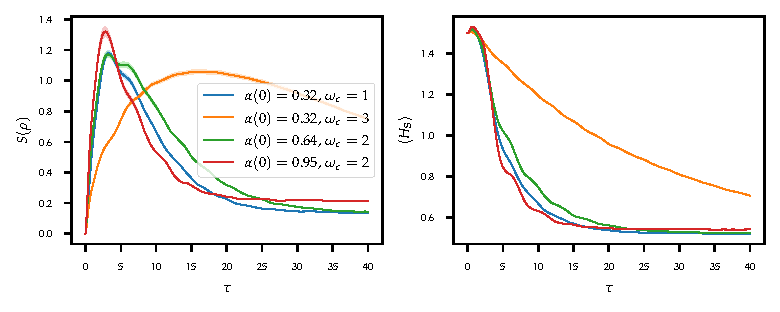
\includegraphics{figs/analytic_comp/entropy_zero.pdf}
  \caption{\label{fig:ho_zero_entropy} Left panel: The von Neumann
    entropy of the system state as a measure for entanglement with the
    bath. Right panel: The system energy as a function of time. The
    \(ω_{c}=3\) case (orange) is markedly different from the others,
    with a much slower decay of the system energy and slower entropy
    dynamics. The strongest coupling simulation (red) converges to a
    markedly different steady state.}
\end{figure}
The ``backflow'' observed in \cref{fig:comp_zero_t} for stronger
coupling seems to diminish the advantage of stronger coupling over
larger bath memories. The decay of the red curve in the right panel of
\cref{fig:ho_zero_entropy} is barely faster than the decay of the blue
curve, despite much larger coupling strength in the case of the red
curve. This may be due to the system interaction ``too long'' with a
given portion of the bath. Here we observe this behaviour for stronger
coupling which shortens the time-scale of energy exchange. In
\cref{sec:one_bath_cutoff} we will see, that these oscillations occur
generically for long bath memories and stronger coupling, and that
energy transfer performance is strongly dependent on timing.

Note however, that the steady state is not a product state as can be
seen by the residual entropy in \cref{fig:ho_zero_entropy} in the
cases where the steady state has been approximately reached. The
stronger the coupling, the larger the entanglement. The \(α(0)=0.95\)
simulation appears to be leading to a qualitatively different steady
state than the one with the same cutoff but weaker coupling
strength. This also manifests in a higher expected system energy in
the steady state.

The time dependence of the entropy the expectation value of the system
energy is markedly different for \(ω_c=3\). Although the coupling
strength is larger than in the \(α(0)=0.32,\, ω_c=1\) case the energy
loss of the system is much slower and the initial energy gain is
less pronounced. This is consistent with the flow in
\cref{fig:comp_zero_t}.

The simulation was run with a hierarchy depth of \(\norm{\vb{k}} \leq 5\)
(simplex truncation\footnote{see \cref{sec:hops_basics}}) and a BCF
fit with \(7\) terms taken from \cite{RichardDiss} which was also used
in the analytical solution. The harmonic oscillator Hilbert space was
truncated to \(15\) dimensions. As the initial state the first excited
state of the oscillator was chosen. Some \(N=5000\) trajectories have
been computed and lead to a quite satisfactory statistical error that
is small enough to be invisible in \cref{fig:comp_zero_t}. The
normalized standard deviation of the bath energy flow follows the
usual one-over-square-root rule as is illustrated in
\cref{fig:sqrt_conv}. Even after just \(N=1000\) trajectories the
relative statistical error is on the order of \(10^{-3}\).
\begin{figure}[h]
  \centering
  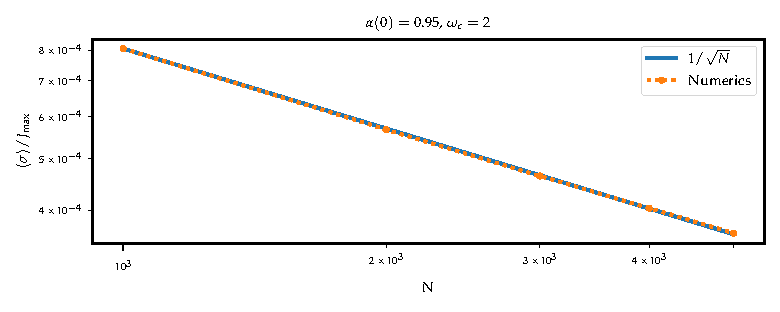
\includegraphics{figs/analytic_comp/sqrt_convergence.pdf}
  \caption{\label{fig:sqrt_conv} The (empirical) standard deviation
    (the statistical error) of the flow for the last configuration in
    \cref{fig:comp_zero_t} normalized by the maximum absolute value of
    \(J\). The \(1/\sqrt{N}\) rule is obeyed to good accuracy showing
    that the estimation of the variance is sound.}
\end{figure}
\begin{figure}[h]
  \centering
  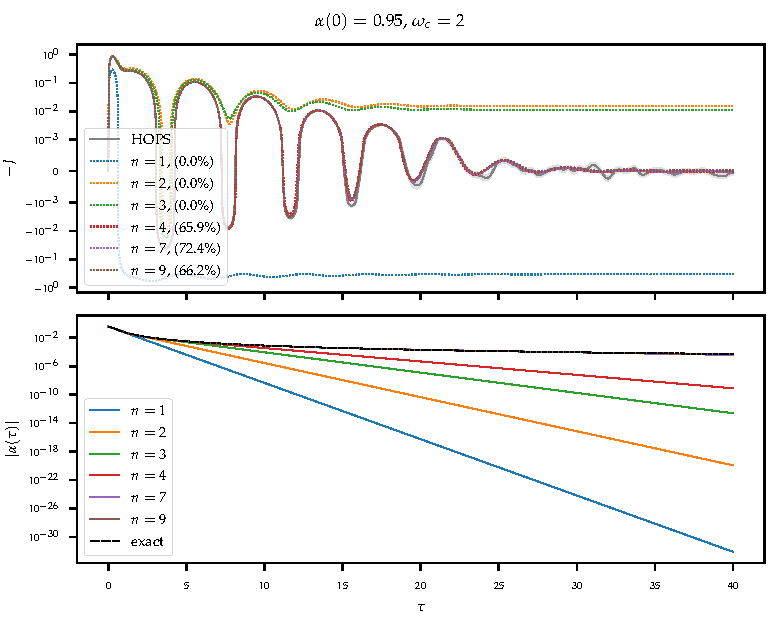
\includegraphics{figs/analytic_comp/analytical_terms_important.pdf}
  \caption{\label{fig:analytical_terms_important} Upper Panel: The
    analytical solution for the zero temperature bath energy flow
    using different numbers of terms in the BCF expansion in a
    symmetric logarithmic scale. For \(7\) terms the consistency
    (number in parentheses) with the numerical solution is best. For
    \(n<4\) the results are unphysical in the steady state.  Lower
    Panel: The absolute value of the approximated bath correlation
    function.}
\end{figure}

The analytical solution is quite sensitive to the quality of the BCF
expansion.  While one might expect that choosing the same number of
terms in the expansion for the analytical solution as was used for the
HOPS simulation, there still remains a systematic difference between
HOPS and the analytical solution, as the stochastic processes is
sampled using the full bath correlation function and applying more
intricate numerical approximations~\cite{RichardDiss}.  Nevertheless,
the best agreement is found for using the same number expansion terms
in both HOPS and the analytical solution as is illustrated in
\cref{fig:analytical_terms_important}. Note that the consistency value
given in \cref{fig:analytical_terms_important} is slightly different
from the one in \cref{fig:comp_zero_t}, as here a separate fit was
made rather than using the fit from \cite{RichardDiss}.

Interestingly, the solutions using a BCF expansion with three terms or
fewer lead to an unphysical non-zero steady state bath energy
flow. Considering specifically the case of one expansion term this may
be related to the fact that now the BCF term so that
\(α(τ)=G \exp(-Wτ)\) is related to a Lorentzian spectral density that
also includes unphysical negative frequencies. To correctly reproduce
the steady state, the fit must model the decay of the BCF correctly on
the appropriate time scales.
\fixme{additional curve in plot, idea: start in the zero state ->
  product state is not the steady state, maybe longer times}

\paragraph{Finite Temperature}
\begin{figure}[t]
  \centering
  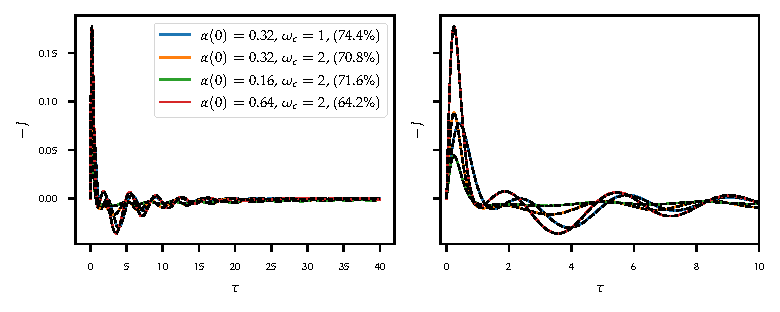
\includegraphics{figs/analytic_comp/flow_comp_nonzero.pdf}
  \caption{\label{fig:comp_finite_t} The bath energy flow \(-J\) of
    the quantum Brownian motion model for different parameters of the
    ohmic bath correlation function \cref{eq:ohmic_bcf} in the finite
    temperature \(T=1\) case. The presentation is equivalent to
    \cref{fig:comp_zero_t}.}
\end{figure}
The results for the finite temperature case are illustrated in
\cref{fig:comp_finite_t} for a temperature of \(T=1\). The setup was
otherwise equivalent to the zero temperature simulations, except for
the number of trajectories which was chosen to be \(N=10^5\).  Again
the high consistency values suggest that the findings of
\cref{chap:flow} are valid. The last case (\(α(0)=0.64,\, ω_c=2\)),
falls just short of the \(68\%\) mark, but agrees very well
visually. It is very probable, that simply more samples are
required.\fixme{maybe re-run...}

We find a similar behaviour to the zero temperature case, but this
time with a more pronounced flow out of the bath as it has a nonzero
energy expectation value. For higher coupling strengths, the flow
amplitude is higher, as is also the case for lower cutoffs.

One potentially contestable point in \cref{chap:flow} was the
appearance of the time derivative of the thermal stochastic process in
\cref{eq:pureagain}. The numerical method which is used to sample the
stochastic processes allows for a straight forward implementation of
this derivative so that no numerical derivatives are required and
there appears to be no problem.

As the dimensionality of the Monte Carlo integral underlying the
NMQSD/HOPS formalism is increased by the ``Stochastic Hamiltonian''
method, we observe markedly slower convergence as the variance of the
individual trajectories is higher. In \cref{fig:cons_dev_finite} the
convergence behaviour, as well the consistency with increasing
trajectory count are plotted and this behaviour is observed. We also
find that in the more challenging regimes of stronger coupling or
longer bath correlation times the behaviour of the convergence is more
volatile, dipping into regions of inconsistency even at high sample
counts. While the mean difference between the numerical and the
analytical flow is always below the mean statistical error, larger
fluctuations can occur at certain points in time when a new region of
the probability space is sampled.

\begin{figure}[p]
  \centering
  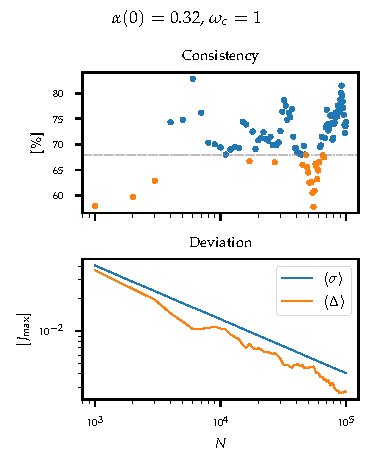
\includegraphics{figs/analytic_comp/consistency_development_0.pdf}
  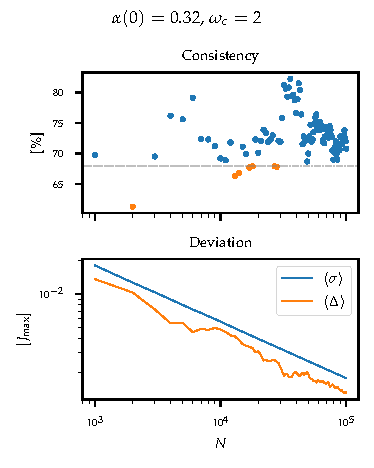
\includegraphics{figs/analytic_comp/consistency_development_1.pdf}
  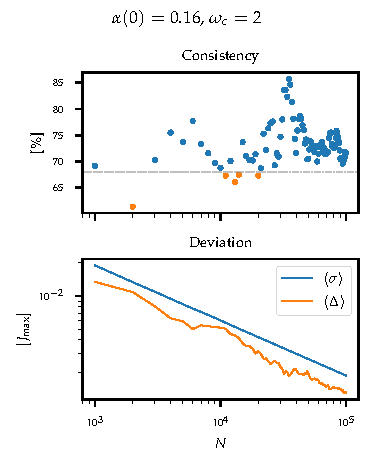
\includegraphics{figs/analytic_comp/consistency_development_2.pdf}
  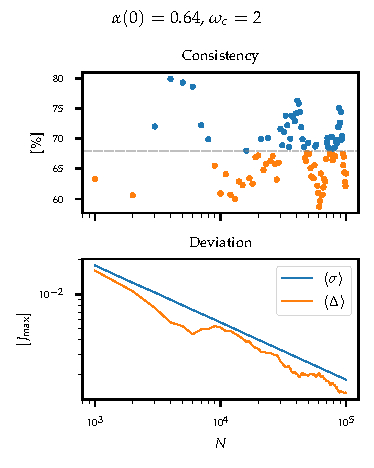
\includegraphics{figs/analytic_comp/consistency_development_3.pdf}
  \caption{\label{fig:cons_dev_finite} The convergence of the flows of
    \cref{fig:comp_finite_t} with increasing trajectory count. The
    upper panels show the consistency, where the grey line marks the
    \(68\%\) threshold for consistency. The lower panel shows the time
    averaged values of the statistical error \(\ev{σ}\) and the
    deviation from the analytical result \(\ev{Δ}\) by the maximum
    absolute value of \(J\). In the last plot, the consistency
    development is quite unstable despite the mean deviation from the
    analytical result being smaller than the mean standard
    deviation. In all cases these two curves scale with the
    \(1/\sqrt{N}\) rule.}
\end{figure}

% The advantage of the ``Stochastic Hamiltonian'' method for finite
% temperature (see \cref{eq:thermalh}) is that one doesn't have to deal
% with the finite temperature BCF that does decay markedly slower than
% its zero temperature counterpart as is illustrated in
% \cref{fig:bcf_decay}. Generically, more terms in the BCF expansion
% would be required to capture the algebraic decay appropriately.

% \begin{figure}[t]
%   \centering
%   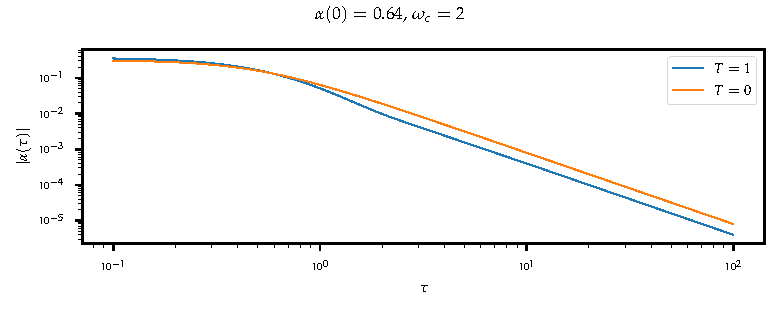
\includegraphics{figs/analytic_comp/bcf_decay.pdf}
%   \caption{\label{fig:bcf_decay} The absolute value of the Ohmic BCF
%     used in the last simulation of \cref{fig:comp_zero_t}.}
% \end{figure}

\subsection{Two coupled Harmonic Oscillators coupled to two Baths}
\label{sec:twoosccomp}
We now progress to a slightly more complicated setting, namely that of
two oscillators coupled to two baths\footnote{This also constitutes
  the first application of the TU-Dresden TQO group's HOPS code-base
  to multiple baths.}. As noted before, multiple baths are an
important ingredient for interesting models like quantum-thermodynamic
engines. At the same time, this setting is much more numerically
challenging as the number in BCF expansion terms doubles, which in
turn increases the number of hierarchy states.

The model of \cref{sec:oneosc} was generalized to two oscillators
coupled to two separate baths in \cref{sec:twoosc} and
\cref{eq:hamiltonian_two_bath}. In this section we simulate this model
and compare the results with the analytical solution.

For simplicity, the parameters were chosen symmetric so that the
frequencies of both oscillators are the same \(Ω=Λ=1\). As before,
\(Ω\) defines the energy unit. The zero temperature bath correlation
functions of both baths were chosen identically with a cutoff
frequency \(ω_c=2\). The intra-oscillator coupling was chosen as
\(γ=0.5\). The hierarchy was truncated so that \(\abs{\vb{k}}\leq 3\) and a BCF
expansion with five terms was chosen to limit memory demands and
\(10^{4}\) trajectories were integrated.

To limit the variance the temperature of one of the baths was set to
zero, so that only one thermal stochastic process was introduced. The
other bath was chosen to have \(T=0.6\). The ground state of the
system Hamiltonian \(\ket{0}\otimes \ket{0}\) was chosen as the
initial state of the oscillators.

The main challenge of simulating the model \cref{eq:hamiltonian_two_bath} is
the dimension of the system Hilbert space which is constrained by the
available memory. In the simulation discussed here, each oscillator
was truncated at \(9\) levels leading to \(9^2 = 81\) dimensions in
total\footnote{This is a naive method of truncation, but sufficient
  for the purposes of this work.}. The effect of a too drastic
truncation of the system Hilbert space can be seen in
\cref{fig:insufficient_levels}. At the temperature chosen the mean
level occupation of a harmonic oscillator is given by the Bose distribution
\begin{equation}
  \label{eq:harm_mean_occ}
  \ev{n} = \frac{1}{\eu^{Ωβ}-1} \approx 0.23 < 1.
\end{equation}
Nevertheless, quite more than two levels are required per
oscillator. This may be due to a required minimal resolution of the
position operators that occur in the model
\cref{eq:hamiltonian_two_bath} which is formulated with position space
in mind.

The final result can be studied in \cref{fig:sufficient_levels}. We
find good, but not excellent agreement. Based on the results of
\cref{sec:oneosccomp} however, it can be argued that this result is
sufficient to corroborate the validity of the results of
\cref{sec:multibath}. With more computational effort\footnote{Mainly
  more BCF expansion terms.} and fine-tuning of parameters an even
better agreement between the analytical and the numerical results may
be achieved.
\begin{figure}[h]
  \centering
  \begin{subfigure}[t]{.49\linewidth}
    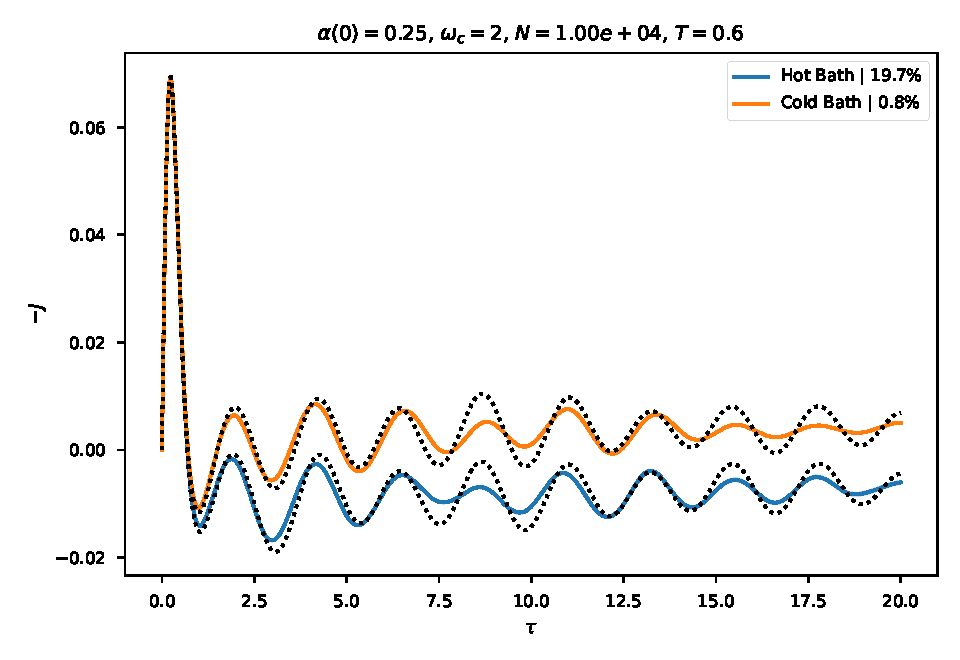
\includegraphics{figs/analytic_comp/comparison_two_5bcf_5ho.pdf}
    \caption{\label{fig:insufficient_levels}\(\dim\hilb_\sys=25\).}
  \end{subfigure}
  \begin{subfigure}[t]{.49\linewidth}
    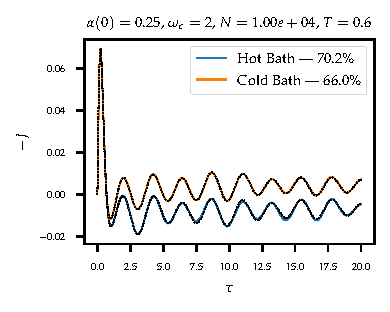
\includegraphics{figs/analytic_comp/comparison_two_ho.pdf}
    \caption{\label{fig:sufficient_levels}\(\dim\hilb_\sys=81\).}
  \end{subfigure}
  \caption{\label{fig:comp_two_bath} The bath energy flows for
    the model \cref{eq:hamiltonian_two_bath}, where the dashed lines
    correspond to the analytical solutions.}
\end{figure}

\Cref{fig:comp_two_bath} exhibits some interesting features. The
initial slip peak in the bath energy flows is identical for both baths
and independent of temperature as suggested by the discussion in
\cref{sec:pure_deph}. As is expected, the hot bath looses energy and
the cold bath gains energy, while this process is modulated by the
intra-oscillator coupling. It follows from the analytical solution
that eventually a steady state without oscillations will be reached.

The zero temperature bath flow converges very much faster than the
finite temperature flow despite the whole system being connected, at
least indirectly, to the hot bath. The reason for this is that the
derivative of the thermal stochastic process \(\dot{ξ}\) dominates the
variance of the flow for each trajectory. This is also the reason that
expressions depending on the hierarchy states rather than time
derivatives of stochastic processes are preferred as discussed in
\cref{sec:general_obs}.

We have shown that the findings of \cref{chap:flow} are consistent
with \cref{chap:analytsol} and that through a careful choice of the
HOPS parameters such as hierarchy depth, Hilbert space dimension and
BCF expansion the exact open system dynamics of the bath energy flow
can be reproduced. The statistical error can be made arbitrarily small
by increasing the trajectory count. For a given target error, the
trajectory count can be estimated by the empirical standard deviation
of a given observable.

For future work there remains the generalization of the work in this
section and \cref{chap:analytsol} to time dependent couplings and
Hamiltonians. Because the NMQSD and also HOPS are largely agnostic of
these factors, we may safely assume that the results of the comparison
will be similar to the ones presented here.

\section{Pure Dephasing and The Initial Slip}
\label{sec:pure_deph}
As seen in \cref{fig:comp_finite_t,fig:comp_zero_t,fig:comp_two_bath},
the short time behavior of the bath energy flow is dominated by
characteristic peak at short times. Because this peak occurs at very
short time scales, it may in part be explained by a simple calculation
which neglects the system dynamics by setting \(H_\sys=0\).

We solve the model with the Hamiltonian (Schr\"odinger picture)
\begin{equation}
  \label{eq:puredeph}
  H = L^†(t) B + L(t) B^† + H_\bath
\end{equation}
with \(L(t)=L(t)^†\), \([L(t), L(s)] = 0\;\forall t,s\) (so that
Heisenberg Hamiltonian matches \cref{eq:puredeph}) and \(B,\,H_\bath\)
as in \cref{sec:nmqsd_basics}.

Because \([L,H]=0\) we can immediately solve \(L_H(t)=L_S(t)\), where
the subscript distinguishes the Heisenberg and Schr\"odinger pictures
respectively. The Heisenberg equations for the \(a_λ\) yield
\begin{equation}
  \label{eq:alapuredeph}
  a_λ(t) = a_λ(0) \eu^{-\iu ω_λ  t} - \iu g_λ^\ast∫_0^t\dd{s} L(s)
  \eu^{-\iu ω_λ  (t-s)}.
\end{equation}

This allows us to calculate
\begin{equation}
  \label{eq:pureflow}
  \dot{H}_\bath = - ∑_λ g_λ L(t) \qty[∂_t a_λ(0) \eu^{\iu ω_λ t} - \iu
  g_λ^\ast∫_0^t\dd{s} L(s) ∂_t \eu^{-\iu ω_λ (t-s)}] + \hc,
\end{equation}
which gives with a state of the form \(ρ=\ketbra{ψ} \otimes ρ_β\)
(\(ρ_β\) being a thermal state)
\begin{equation}
  \label{eq:pureflowexpectation}
  \ev{\dot{H}_\bath } = -2 ∫_0^t\dd{s}\ev{L(t)L(s)} \Im[\dot{α}(t-s)].
\end{equation}
For time independent \(L\) this becomes
\begin{equation}
  \label{eq:pureflowtimeindep}
  \ev{\dot{H}_\bath } = -2 \ev{L^2} \Im[α(t)].
\end{equation}

The proportionality to the imaginary BCF \(α\) does explain the
initial peak in the bath energy flow. The imaginary part of the BCF is
zero for \(t=0\) and then usually features a peak at rather short
times (assuming finite correlation times). For the ohmic BCF used here
and shown in \cref{fig:ohm_bcf_ex}, this feature is very prominent.
\begin{figure}[h]
  \centering
  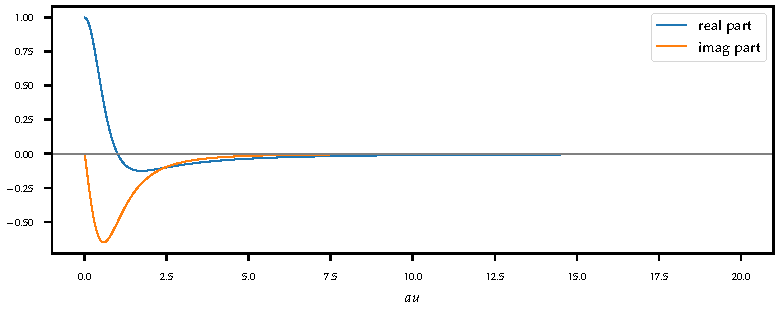
\includegraphics{figs/misc/ohmic_bcf_example.pdf}
  \caption{\label{fig:ohm_bcf_ex} An ohmic BCF with \(ω_{c}=η=1\). The
  imaginary part has a peak at the beginning and decays to zero.}
\end{figure}

Generically, the imaginary part of the BCF is negative at least for
short times as it takes the form
\begin{equation}
  \label{eq:negtive_imag}
  \Im[α(τ)] = -\frac{1}{π}∫_{0}^{τ}J(ω) \sin(ωτ)\dd{ω}
\end{equation}
which is negative for \(τ\leq π/ω_{\mathrm{max}}\), where
\(ω_{\mathrm{max}}\) is a characteristic cutoff frequency of the
system. The direction of the initial slip flow for unmodulated systems
will therefore be always be into the bath compensating for negative
interaction energy.

Interestingly, \cref{eq:pureflowexpectation} does not contain any
reference to the temperature of the bath. Therefore, the bath energy
can only surpass its initial value in this model, as the dynamics
match the zero temperature case in which the bath has minimal energy
in the initial state.

A thermodynamically useful model should feature significant system
dynamics that do not commute with the interaction or modulation so
that the Hamiltonian does not commute with itself at different
times. Coupling that is not self-adjoint \fixme{plot: if time, i could
  do the energy shovel with non-hermitian} may also have this effect,
but in the literature most effective qubit models tend to favour
Hermitian couplings
\cite{Aurell2019Apr,Hita-Perez2021Nov,Hita-Perez2021Aug,MacQuarrie2020Sep,Andersen2017Feb,Mezzacapo2014Jul}. For
the spin-boson system, non Hermitian coupling it is the result of the
random phase approximation, which however does not imply weak
coupling~\cite{Irish2007Oct}.

For completeness, the interaction energy is given by
\begin{equation}
  \label{eq:pureinter}
  H_\inter = L(t)\qty[∑_λg_λ\qty(a_λ(0)\eu^{-\i ω_λ t} - \i
  g^\ast_λ∫_0^t\dd{s} L(s) \eu^{\i ω_λ (t-s)})] + \hc,
\end{equation}
yielding
\begin{equation}
  \label{eq:pureinterexp}
  \ev{H_\inter} = 2 ∫_0^t\dd{s}\ev{L(t)L(s)} \Im[α(t-s)].
\end{equation}

For time independent coupling we have
\begin{equation}
  \label{eq:pureinterexp_timeidp}
  \ev{H_\inter} = 2 \ev{L^2} \int_{0}^{t}\Im[{α}(s)]\dd{s} = -Δ\ev{H_{\bath}}.
\end{equation}

It may be useful to normalize the BCF based on \cref{eq:pureinterexp},
so that the pure interaction energy build-up in the initial slip is
taken as measure of interaction strength. To make the normalization
independent of \(L(t)\), we choose the normalization to be
\begin{equation}
  \label{eq:bcfnorm}
  \begin{aligned}
  \mathcal{N} &= 2 \abs{\frac{\max_t\norm{L(t)L^\dag(t)+\hc}}{\max_t{\norm{H(t)}}} ∫_0^∞ \Im[α_u(τ)]\dd{τ}}\\
    α(τ) &= α_u(τ)/\mathcal{N},
  \end{aligned}
\end{equation}
where \(α_u\) is some unnormalized BCF. This normalization has the
useful property, that it neutralizes any scaling in \(L\). Note that
here the convention in which \(α\) is dimensionless is used.

% this is not true
% imaginary part becomes proportional to the Dirac delta in the limit
% where typical cutoff frequency \(ω_c\rightarrow ∞\). The integral over
% the real part of \(α\) always gives zero if the spectral density obeys
% \(J(0) = 0\) and tends to exhibit fast oscillations and fast decay in
% the large-cutoff limit. For weak coupling, it may therefore be
% neglected. This constitutes the Markov limit mentioned in
% \cite{Strunz2001Habil}.
The Ohmic-type BCF is
\begin{equation}
  \label{eq:normohmic}
  α(τ)=\frac{ω_c  s }{ (\max_t\norm{H})(1+\iu ω_c τ)^{s+1}},
\end{equation}
in this normalization.

\section{Precision Simulations of the Zero Temperature Spin-Boson Model}
\label{sec:prec_sim}
\begin{itemize}
\item often no analytical solution available: how to verify
  convergence?
\item at the same time: simplest model to start with, numerically
  simple
\item good starting point to get to know the system and find out if
  results can be trusted
\end{itemize}

Despite being solvable analytically, the models from
\cref{sec:hopsvsanalyt} are numerically cumbersome, as their system
Hilbert space is infinite dimensional and has to be truncated. In this
section we concern ourselves with a very simple model that poses
lesser numerical challenges and still exhibits interesting behaviour.

Both the performance of the HOPS method itself
(\cref{sec:stocproc,sec:trunc}) and the characteristics of the flow
mediated by the concrete form of the bath correlation function
(\cref{sec:one_bath_cutoff,sec:one_bathcoup_strength}) will be
investigated. We will find that the numerics do indeed yield very
consistent results and that the specifics of the energy flow depend
very much on the spectral density.

As an analytical solution to a given open system is generally not
known, another indicator of the proper choice of HOPS parameters is
required. Upon the example of a single qubit coupled to a single zero
temperature bath, we will study the convergence behaviour of the
interaction energy.  The corresponding Hamiltonian is
\begin{equation}
  \label{eq:one_qubit_model}
  H = \frac{1}{2} σ_z + \frac{1}{2} ∑_λ\qty(g_λ σ_x^† a_λ + g_λ^\ast
  σ_x a_λ^†) + ∑_λ ω_λ a_λ^\dag a_λ,
\end{equation}
where we have chosen \(H\) to be dimensionless\footnote{The energy scale
is set by the system Hamiltonian.}.

In the language of HOPS this corresponds to \(H_\sys=σ_z/2\),
\(L=σ_x/2\). We again choose the Ohmic BCF as explained in
\cref{sec:meth}. Throughout this section we choose the ``up'' state
\(H_S\ket{1} = 1/2\ket{1}\) as the initial state of the system.

The main measure of convergence for variables other than the
trajectory count are consistency conditions. One check available to us
is energy conservation which allows us to calculate the expectation
value of the interaction energy through integration of the bath energy
flow. The interaction energy obtained in this way can then be compared
to the interaction energy obtained directly as shown in
\cref{sec:intener}. Note that this scheme may also be adapted easily
to multiple baths where the sum of interaction energies has to be
considered and to time dependent Hamiltonians where finite power has
to be taken into account.

The main sources of systematic deviations for the model
\cref{eq:one_qubit_model} are the quality of the sampling of the
stochastic process and the cutoff of the hierarchy. The first becomes
important when the cutoff frequency is large and the BCF vanishes
rapidly and has to be resolved on shorter time scales. The second is
important when the cutoff frequency is smaller and the bath has a
longer memory.

\subsection{Stochastic Process}
\label{sec:stocproc}
For studying the convergence behaviour regarding the sampling of the
stochastic process we chose the cutoff as \(\norm{\vb{k}} \leq 4\)
(simplex truncation\footnote{see \cref{sec:hops_basics}}),
\(N=4.5 \cdot 10^5\) trajectories and an Ohmic BCF with \(α(0)=1.6\)
and \(ω_c=4\).  The sampling method uses the ``Fast Fourier
Transform'' (FFT) as described in~\cite{RichardDiss}. As the system
Hilbert space dimension is small, a BCF expansion with seven terms was
employed.

The main parameter of this method is the accuracy of the FFT. The
implementation compares the BCF and its FFT approximation on the time
interval of the simulation and chooses the internal
parameters\footnote{The number of time grid points and the integral
  boundaries in frequency space.} so that the difference normalized by
\(α(0)\) is smaller than a given value \(ς\).

\begin{figure}[h]
  \centering
  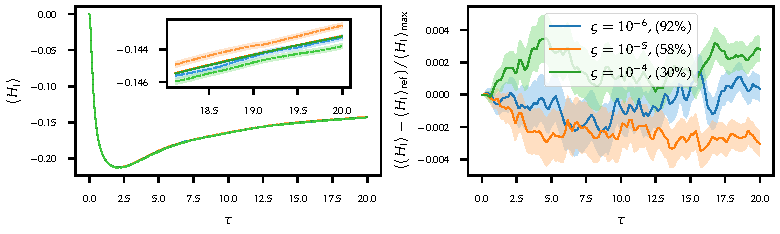
\includegraphics{figs/one_bath_syst/stocproc_systematics_interaction}
  \caption{\label{fig:stocproc_systematics} Left panel: The
    interaction energy of the model \cref{eq:one_qubit_model} for
    \(α(0)=1.6\) and \(ω_c=4\) using different precisions for the
    sampling of the stochastic process. The dashed lines are obtained
    using energy conservation while the solid lines are obtained
    directly as in \cref{sec:intener}. The consistency between the two
    is given in the legend of the right panel. An inset shows the
    curves for the final three time units. Right panel: The difference
    of the interaction energies obtained using energy conservation and
    directly. The values are normalized by the maximal absolute value
    of the interaction energy. The \(\varsigma = 10^{-6}\) case gives
    the most accurate results in terms of energy conservation, but
    when using the direct method of calculating \(\ev{H_{\inter}}\)
    all parameter choices yield the same results.}
\end{figure}
\Cref{fig:stocproc_systematics} illustrates the effect of this
parameter. We find very good qualitative agreement for all values of
\(ς\). The indirectly calculated value of then interaction energy
shows some fluctuation between the settings, but the value calculated
directly is very stable as can bee seen in the inset of
\Cref{fig:stocproc_systematics}.

Only in the \(\varsigma=10^{-6}\) case however, compatibility is
satisfied at the given sample count. This is due to the fact that here
multiple values that are obtained in different ways, namely system
energy and the flow, have to be considered. The system energy depends
on the zeroth hierarchy order only whereas the flow additionally
depends on the first hierarchy states and has to be numerically
integrated.
\begin{figure}[htp]
  \centering
  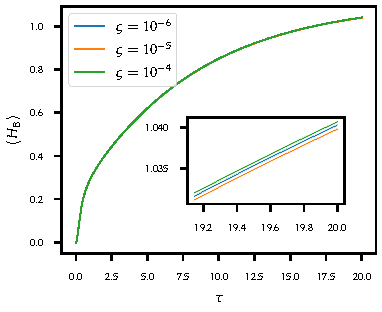
\includegraphics{figs/one_bath_syst/stocproc_systematics_bath_energy}
  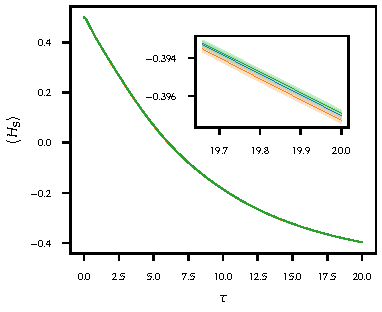
\includegraphics{figs/one_bath_syst/stocproc_systematics_system}
  \caption{\label{fig:stocproc_bath_sys}The bath and system energies of the
    model \cref{eq:one_qubit_model} for \(α(0)=1.6\) and \(ω_c=4\)
    using different precisions \(\varsigma\) for the sampling of the
    stochastic process. Systematic deviations outside the error bounds
  occur mainly in the bath energy.}
\end{figure}

The individual contributions to the indirectly obtained interaction
energy may be studied in \cref{fig:stocproc_bath_sys}. The bath
energy, being an integrated quantity for which errors may accumulate,
is most susceptible to systematic deviations outside the error bounds,
as is clearly visible in the insets. Nevertheless, the qualitative
agreement of the different simulations is excellent.

The development of the consistency of trajectory count \(N\) can be
studied in \cref{fig:stocproc_consistency_dev}. Only for the highest
precision case we have a consistent picture. For lower precision, the
consistency fluctuates and only occasionally surpasses \(68\%\). For
the lower precisions we find that they initially demonstrate
compatibility (until about \(N=10^4\)) but eventually diverge from the
exact\footnote{The result that demonstrates compatibility
  consistently.} result. It is therefore important to consider the
dependence of the compatibility on the sample count \(N\) to judge the
veracity of the simulation results.
\begin{figure}[htp]
  \centering
  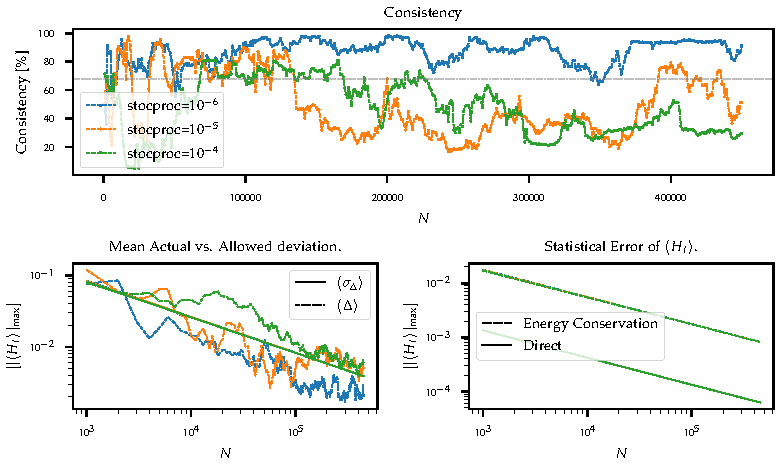
\includegraphics{figs/one_bath_syst/stocproc_systematics_consistency}
  \caption{\label{fig:stocproc_consistency_dev} Upper panel: The
    compatibility (number of values within one standard deviation, see
    \cref{sec:meth}) of the flow (direct computation vs. energy
    conservation) of the model \cref{eq:one_qubit_model} for
    \(α(0)=1.6\) and \(ω_c=4\) using different precisions
    \(\varsigma\) for the sampling of the stochastic process in
    relation to the trajectory count \(N\). Only the
    \(\varsigma=10^{-6}\) simulation is consistent for all sample
    counts. Lower left: The time averaged difference of the direct and
    indirect interaction energies (dashed) and the time averaged
    standard deviation of the difference (solid) as a function of
    trajectory count. Only for the smallest \(\varsigma\) the
    difference is consistently smaller than the standard deviation of
    the difference. Lower right: The time averaged statistical errors
    of the interaction energy calculated directly (solid lines) and
    indirectly through energy conservation (dashed lines). The
    deviation of the direct method smaller by an order of magnitude.}
\end{figure}

Apart from being closer to the correct result, the direct computation
of the interaction energy has the advantage of providing faster
convergence\footnote{See \cref{fig:stocproc_consistency_dev}, lower right
  panel.}.

\subsection{Hierarchy Truncation}
\label{sec:trunc}
As the effect truncation depth has already been studied thoroughly
in~\cite{RichardDiss}, we will keep the discussion short.  We chose
\(N=4.5 \cdot 10^5\) trajectories and an Ohmic BCF with \(α(0)=0.8\)
and \(ω_c=2\). Again, seven a BCF expansion with seven terms have been
used. The coupling strength has been chosen with the help of
\cref{sec:pure_deph}, so that the interaction energy is of a similar
order of magnitude as in the discussion
above. \Cref{fig:k_systematics} suggests that there seems to be no
improvement in accuracy or even change in the value of the flow for
\(\norm{\vb{k}}\geq 4\). However, the inset in the left panel
demonstrates that the direct result differs slightly for
\(\norm{\vb{k}} = 2\), which demonstrates that an adequate choice of
truncation depth is important.
\begin{figure}[htp]
  \centering
  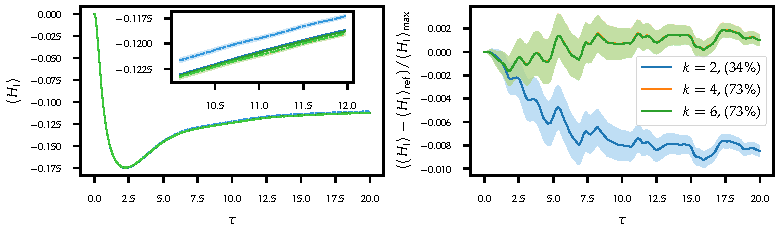
\includegraphics{figs/one_bath_syst/k_systematics_interaction}
  \caption{\label{fig:k_systematics} The same as
    \cref{fig:stocproc_systematics} but for \(α(0)=0.8\) and
    \(ω_c=2\) and for various truncation depths \(k=\norm{\vb{k}}_{\mathrm{max}}\).}
\end{figure}


We see in \cref{fig:k_systematics_system} that the difference of the
\(\norm{\vb{k}} = 2\) case from the \(\norm{\vb{k}} = 6\) is on the
same order of magnitude for system energy and interaction energy. The
bath energy, being an integrated quantity, accumulates errors and
deviates the most. Also, the results for \(\norm{\vb{k}} = 4,6\) agree
perfectly in all cases.
\begin{figure}[htp]
  \centering
  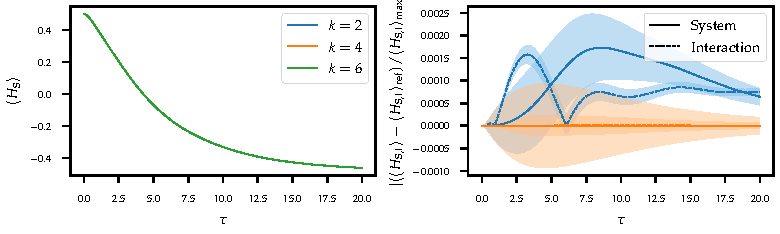
\includegraphics{figs/one_bath_syst/k_systematics_system}
  \caption{\label{fig:k_systematics_system} Left panel: The norm of
    the difference of a single trajectory to the \(\norm{\vb{k}} = 6\)
    case. The solid lines show the difference of the zeroth hierarchy
    states and the dashed lines show the same for the first hierarchy
    states.  There is still a slight difference on the trajectory
    level. Right panel: The difference between the \(k=6\) result and
    the results with \(k<6\) normalized by the maximal absolute system
    energy (solid lines) and the same for the interaction energy
    (dashed lines) as well as the bath energy change (dotted). The
    deviation is most substantial for the bath energy change, as
    errors can accumulate in the integration of the bath energy flow.}
\end{figure}
The left panel of \cref{fig:k_systematics_system} demonstrates, that there is still a
difference greater than the machine epsilon on the level the
trajectories. This difference however, is small enough not to impact
observables much.  The deviation of the system, interaction and bath
energies from the highest precision case (\(k=6\)) is also
plotted.


Summarizing, we conclude that the HOPS parameters have to be chosen
carefully for precision simulations, but that a more relaxed choice of
parameters already give a \emph{very} good qualitative picture.

\fixme{maybe run a simulation with more hierarchy depth and more bcf
  terms, check whether there is a mistake} It remains for future work
to perform a detailed study of the systematics of the finite
temperature flow and modulated Hamiltonians. In the following sections
we will look at some examples of physically interesting systems with
less focus on the systematics of convergence.

\subsection{Varying the Cutoff Frequency}
\label{sec:one_bath_cutoff}
The lessons learned in \cref{sec:stocproc,sec:trunc} will now be
applied to simulate \cref{eq:one_qubit_model} with high consistency
for various parameter choices of the cutoff \(ω_{c}\) of the BCF
\begin{equation}
  \label{eq:ohmic_bcf_repeat}
  α(τ) =
  \frac{η}{π}\qty(\frac{ω_c}{1+\iu ω_c τ})^2.
\end{equation}
Guided by these demonstrations, we'll turn to a more detailed analysis
of the role of non-Markovianity in the energy transfer characteristics
of our model. The quantification of the initial slip dynamics in
\cref{sec:pure_deph} will also be verified.

To make the interaction energies comparable to each other, the BCF
normalization of section \cref{sec:pure_deph} is being used. Because
of the small size of the Hilbert space, we were able to choose a HOPS
configuration\footnote{\(\norm{\vb{k}}\leq 7\), seven BCF terms,
  \(\varsigma = 10^{-6}\)} that yields high-accuracy
results\footnote{A detailed account of the consistency is given in
  \cref{fig:omega_interaction_consistency}.}, based on the results of
the previous section. The only problematic result is the one for
\(ω_c=1\), but there is good qualitative consistency in this case.

For all simulations \(N=5\cdot 10^{5}\) trajectories were integrated
to produce the results that are summarized in
\cref{fig:omega_systematics_system}.
\begin{figure}[h]
  \centering
  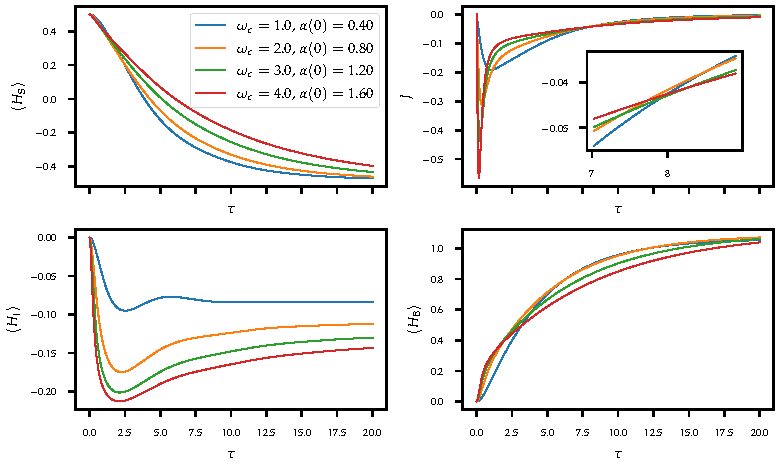
\includegraphics{figs/one_bath_syst/omega_energy_overview}
  \caption{\label{fig:omega_systematics_system} Energy overview for the
    model \cref{eq:one_qubit_model} for various coupling strengths and
     cutoff frequencies. The curves are converged out, and the error
    funnels are not visible.}
\end{figure}

Let us preface the following discussion with a note of caution. All
the discussed phenomena are specific to the minimal model
\cref{eq:one_qubit_model}, although sometimes similarities to
phenomena observed in \cref{sec:hopsvsanalyt} can be seen. Whether
there is some universality to the results obtained is an interesting
question for a more detailed future detailed study.\fixme{Remove this?}

The interaction energy expectation values, despite being in the same
order of magnitude and not in the weak coupling regime, differ
significantly. This illustrates the limitation of the estimate in
\cref{sec:pure_deph} and exemplifies the nontriviality of the open
system dynamics. Better estimates of the interaction energy and thus
interaction strength may be derived from ideas similar to the ones
discussed in \cref{sec:normest}.  Besides the magnitude, the
qualitative time dependence of the interaction energies varies,
especially between the \(ω_c=1\) configuration and the others.

The blue (\(ω_c=1\)) curve exhibits two pronounced turning points in
contrast to the other simulations. This behaviour is a symptom of
interference of the system and bath time scales which are of similar
orders in this simulation, an idea that we will develop further
below. Further, despite having the weakest overall coupling strength
\(α(0)=0.4\) the system energy falls off the fastest after a short
period where it is above the other configurations. This behaviour is
also visible in the bath energy expectation value, where this
simulation almost reaches the same levels as the \(ω_c=2\)
configuration for \(τ\gtrsim 5\).

The flow is generally negative (the bath gains energy) and decays
after an initial peak. All the flow graphs appear to be crossing in
about the same point \(τ\approx 7.7\) after which their ordering by
magnitude is reversed.  The inset shows that the crossing is not
precisely at the same point, nevertheless further investigation of
this phenomenon may of interest in the future. The decay is faster for
higher cutoff frequencies and stronger couplings. Despite the higher
interaction energies and coupling strengths, the high-cuttoff
simulations exhibit a slower energy transfer after the initial peak
has decayed sufficiently, with the system energy falling slower and
the bath energy rising slower. The situation is generally reversed for
short times \(τ\lesssim 2.5\), because here the build-up of
interaction energy is significant.

The presentation in \cref{fig:omega_systematics_system} is not
conducive to comparing the actual performance of the energy transfer,
due to the variable shape of the spectral density and the chosen
coupling strengths. Because the maximum of the Ohmic spectral density
is located at \(ω_c\) the special observed energy transfer behaviour
for \(ω_c=1\) is likely due to a resonance effect (see above) as the
system energy level spacing is unity.

The dissipator of the master equation for this two level system only
depends on the value of the spectral density at the level
spacing~\cite[p. 66]{Rivas2012}\footnote{There \(L=σ_{+}\), but this
  has no bearing on the connection to \(ω_{0}\).}  (\(ω_{0}=1\) here),
so that it is reasonable to expect, that there may be variations
whenever its magnitude at this point changes.  On the other hand, a
strong dependence of the flow on the shape of the bath correlation
function beyond lamb-shift like influences, as we will find below is
an indicator of the departure from the weak coupling limit.
\fixme{Here, some master equation comparison would be nice.}.

\paragraph{Energy Transfer Characteristics}
After focusing on the systematics and achieving very high consistency
in our simulations, we continue to shed some light on the role of bath
memory and resonance in the behavior of the energy transfer between
system and bath.

\begin{wrapfigure}[13]{O}{0.3\textwidth}
  \centering
  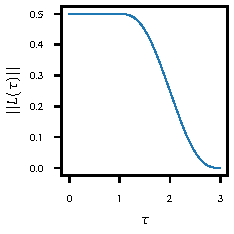
\includegraphics{figs/one_bath_syst/L_mod}
  \caption{\label{fig:L_mod} The smooth modulation of the coupling
    operator \(L(τ)\).}
\end{wrapfigure}
For a systematic study of resonance, we first compare the flow for
shifted ohmic spectral densities\footnote{See \cref{sec:shift_sp} for
  details.} with identical scaling \(α(0)\) and cutoff frequency
\(ω_c=2\). We turn off the interaction smoothly\footnote{A smoothstep
  function of order two with a transition period of two. See
  \cref{sec:smoothstep}.} over two time units before the system has
reached its steady state and compare how much energy has been
transferred in terms of the final bath and system energies and the
loss due to the modulated coupling.

The less energy the system has at the end of the process and the
faster the process concludes, the better the performance of
transfer. If the interaction energies are on the same scale, the
decoupling costs should be roughly the same in terms of total energy
change. Otherwise, they may lead to an additional change of system and
bath energies between the different simulations. Ideally the bath
energy changes to take up any energy added introduced by the
decoupling.

To make space for the shifted bath correlation functions, the system
energy gap has been set to four so that \(α(0)=8\) represents a quite
reasonable coupling strength for our purposes here.

The results for three shifts are presented in
\cref{fig:resonance_analysis}. For all shifts the spectral density has
a finite value at the value of system level spacing, but only in the
\(ω_s=2\) case, the resonance condition is fulfilled. Indeed, the
energy transfer out of the system is the best for the resonant case
(see \cref{fig:resonance_analysis}, middle panel).

The change in total energy due to the decoupling of the bath is
moderately higher than in the resonant case than in the \(ω_s=1\)
case, but the final system energy is the lowest. \fixme{The decoupling
  seems to affect mainly the bath energy (see left panel). Should I
  say so?}
\begin{figure}[htp]
  \centering
  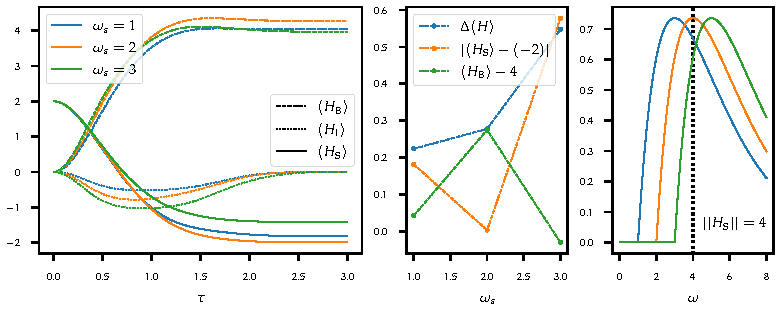
\includegraphics{figs/one_bath_syst/resonance_analysis}
  \caption{\label{fig:resonance_analysis} Left
    panel: The system, bath and interaction energies for various Ohmic
    BFCs with \(α(0)=8,\,ω_c=2\) shifted by \(ω_s\). Mid panel: The
    difference in total energy, the distance of the system energy to
    the ground state energy and the distance of the bath energy to the
    initial system energy. Right panel: The spectral density for the
    three shift values. \(\norm{H_\sys}\) does mean in this case, that
    the energy level spacing of the system is \(4\). There resonant
    case has the best energy transfer behaviour as gauged by the final
    system energy.}
\end{figure}

The third simulation with \(ω_s=3\) exhibits the worst performance
with the highest residual system energy and the highest change in
total energy due the large magnitude of the interaction energy.
Deactivating the interaction lowers the final bath energy in all
cases, but here this effect is most pronounced.

Were the interaction switched off abruptly, the system and bath
energies would remain untouched. Turning the interaction off in finite
time reduces the energy introduced into the system in the cases
discussed here. System and bath energy must therefore compensate part
of the negative interaction energy after the system is decoupled from
the bath. Hence, the observed lowering of system and bath energy after
decoupling. However the effect can also act into the other direction
as we shall see below.

The \(ω_{s}=1\) case exhibits the smallest cost in terms of total
energy change.  The small change in the total energy is due to the
magnitude of the interaction energy, which is the smallest compared to
the other to shifts.

Interestingly, if we modulate the system periodically with angular
frequency \(Δ\), also bath frequencies of \(ω_{0} + n Δ\)
(\(n\in\NN\)) become important, so that shifting the spectral density
to higher frequencies is advantageous, as we will find out in
\cref{sec:modcoup_reso}.

% Turning of the interaction leads mostly to a reduction of the final
% bath energy (see the middle panel).  This effect will also appear in
% most of the cases discussed below. When deriving a master equation for
% this two level system~\cite[p. 68]{Rivas2012}, there occurs a lamb
% shift term that acts as a correction to the unitary evolution of the
% system. Turning the interaction off adiabatically removes this leads
% to a change in what one may define as system energy in this case. In
% the case discussed here, the coupling is not weak so that this
% explanation may only serve as a means of analogy. Compensating for the
% negative interaction energy, the system and bath energy expectation
% value both fall when the coupling is turned off.\fixme{is this
%   reasonable?}

% For an ohmic spectral density the lamb shift energy is
% \begin{equation}
%   \label{eq:lshift_twolevel}
%   2Δ=\eu^{-1/ω_{c}}\,\mathrm{Ei}\qty(\frac{1}{ω_{c}}) - ω_{c},
% \end{equation}
% which is negative for all the cases discussed here and may account for
% some part of the negative interaction energy. In this way, the removal
% of the bath would

\begin{wrapfigure}[16]{O}{0.4\textwidth}
  \centering
  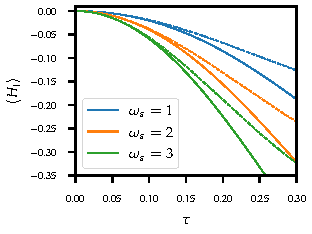
\includegraphics{figs/one_bath_syst/initial_slip_resonance}
  \caption{\label{fig:initial_slip_resonance} The interaction energies
    (solid lines) of the models in \cref{fig:resonance_analysis} and
    the predictions for the interaction energy due to the initial slip
    dynamics \cref{eq:pureinterexp_timeidp} (dashed lines). Larger
    frequency shifts of the spectral density lead to a higher
    magnitude of the interaction energy and faster dynamics.}
\end{wrapfigure}
Generally the maximal absolute interaction energy is roughly
proportional to the shift, so that the short term interaction strength
as measured by the interaction energy expectation value is not only
dependent on the width and total norm of the spectral density, but
also on its absolute distribution in frequency space. The shift adds a
phase factor \(\eu^{-\i ω_{s} τ}\) to the BCF which makes the
imaginary part steeper. This in turn leads to faster initial slip
dynamics and a speed buildup of interaction energy as demonstrated in
\cref{fig:initial_slip_resonance}. The observed effect is sensible on
an intuitive level as higher frequency oscillators are being excited
in the bath leading to faster dynamics.

Due to the asymmetry of the spectral density, the simulations for
\(ω_s=1\) and \(ω_s=3\) are not directly comparable. A repetition of
this investigation with a (pseudo~\cite{Mukherjee2020Jan}) Lorentzian
spectral density and for different interaction
time-frames\footnote{steady state vs. transient states} is left for
future work.

The longer term picture is being studied in
\cref{fig:resonance_analysis_steady}. We see broadly similar energy
transfer characteristics for \(ω_{s}=1\) and \(ω_{s}=2\), where the
off-resonant case may be slightly advantageous. The left panel shows,
that although the system energy before the decoupling is lower in the
resonant case, the situation is reversed during the decoupling as now
also the system energy is affected by the process and the interaction
energy of the off-resonant case is slightly larger in
magnitude. However these effects are quite marginal and should be
taken with care. The system energy difference amounts to
\(\Delta\langle H_\mathrm{S}\rangle=0.00397\pm 0.00010\), but only the
statistical error has been taken into account. The simulations were
run with \(N=10^{4}\) trajectories and the same HOPS settings as in
the discussion above, so that some confidence may be placed in them.

For \(ω_{s}=3\) the approximate steady state has not been reached yet
and the energy transfer is incomplete and the residual system energy
is the highest. The fast growth of the interaction energy leads to a
slower initial loss of system energy. On longer time scales we see a
slow, almost linear transfer of energy from the system into the
interaction. The system dynamics are catching up with the bath.
\begin{figure}[htp]
  \centering
  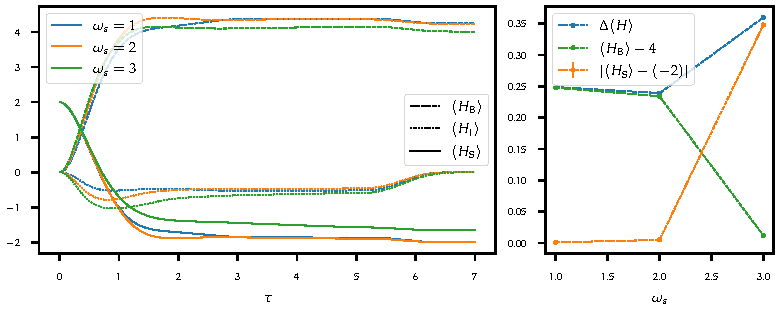
\includegraphics{figs/one_bath_syst/resonance_analysis_steady}
  \caption{\label{fig:resonance_analysis_steady} The same as
    \cref{fig:resonance_analysis} but for a longer coupling time.}
\end{figure}

To study the effect of the bath memory, we use Ohmic spectral
densities with linearly spaced \(τ_{\bath}\equiv ω_c^{-1}\) that have
been shifted and scaled by numerical optimization so that their peaks
coincide and the resulting maximal absolute interaction energies
identical. The rightmost panel of \Cref{fig:markov_analysis} shows
plots of the spectral densities obtained. We can see, that not only
the magnitude at resonance point enters, as the peak heights are quite
different. We will encounter this behavior again in
\cref{sec:extr_mem}.

The results that can be obtained are very much dependent on the
timing. \Cref{fig:markov_analysis} has been arrived at by tweaking the
time point of decoupling so that an extremum in the system energy of
the long memory (\(τ_{B}=1\)) case is captured. This leads to an
advantageous transfer performance with a lower system energy and
similar cost in terms of total energy change, although residual system
energy is still higher than in \cref{fig:resonance_analysis_steady}.
Although initially the system energy falls fastest for the short
memory case the situation is reversed after about \(τ=0.5\).
\cref{fig:resonance_analysis_steady}.
\begin{figure}[htp]
  \centering
  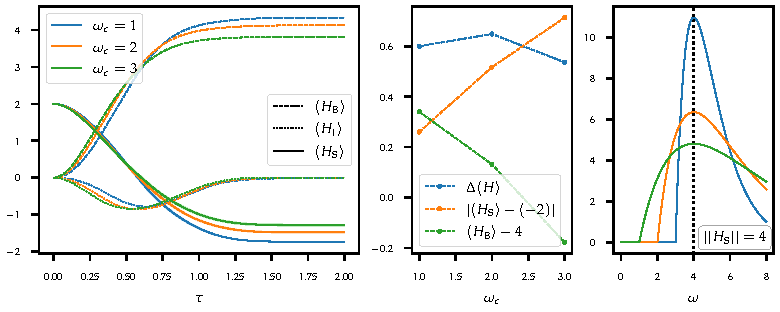
\includegraphics{figs/one_bath_syst/markov_analysis}
  \caption{\label{fig:markov_analysis} The same as
    \cref{fig:resonance_analysis} but for shifted spectral densities
    various bath memory times. The long-memory case performs best in
    this case, exhibiting the lowest final system energy.}
\end{figure}

Because the minimum in the interaction energy of the \(τ_{\bath}=1\)
case comes last, the residual interaction energy and thus interaction
strength is strongest when the interaction is turned off. Therefore
the largest quantity of energy is being introduced into the system in
this case when the interaction is disabled. In all cases the amount of
energy introduced is so large, that the bath energy slightly rises
during the decoupling process instead of falling as in
\cref{fig:resonance_analysis_steady}.


\begin{figure}[htp]
  \centering
  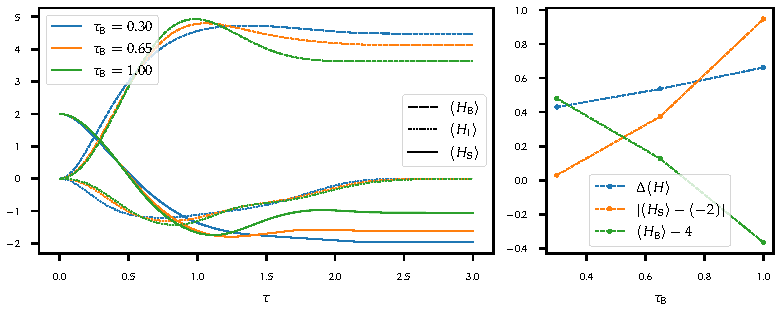
\includegraphics{figs/one_bath_syst/markov_analysis_longer}
  \caption{\label{fig:markov_analysis_longer} The same as
    \cref{fig:markov_analysis} but with slightly different timing. The
    result is exactly the reverse of
    \cref{fig:markov_analysis_longer}. Longer memories perform worse.}
\end{figure}
For slightly longer coupling times but with the same coupling
strengths, we find in the exact opposite picture as can be ascertained
from \Cref{fig:markov_analysis_longer}.  The increased bath memory
time allows for ``back flow'' of energy from the bath into the system
and so the performance of energy transfer is strongly dependent on the
precision of control. The oscillations of flow and thus bath energy
have already been noticed in \cref{sec:oneosccomp} and seem to be a
robust feature of stronger coupling and long bath
memories. \fixme{Append tables for model params.} The total energy
introduced is slightly less than for the short times as the
interaction energy is lower when the interaction is turned off.  The
final bath show an inverse behavior falling as the final system
energies rise. This is due to the energy transfer behavior, consistent
with the broadly similar total energy change in all three cases. This
behavior can also be observed \cref{fig:markov_analysis}.

For even longer times we find a picture similar to
\cref{fig:markov_analysis_steady}. The short memory case shows hardly
any backflow and performs best in terms of final system energy which
is extremely close to the target value of negative two. The other two
bath memories perform worse. We observe that simulation with the
longest bath memory stands out and having a very different final state
as is exemplified by the final system energy and the interaction
energy curve which exhibits a greater magnitude and persistent
oscillations.
\begin{figure}[h]
  \centering
  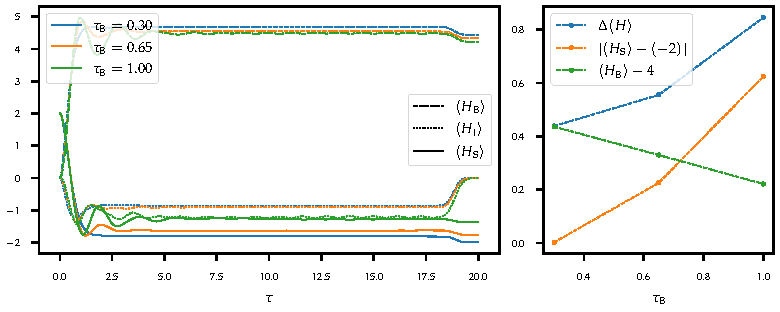
\includegraphics{figs/one_bath_syst/markov_analysis_steady}
  \caption{\label{fig:markov_analysis_steady} The same as
    \cref{fig:markov_analysis} but for long times. The results are
    broadly similar to \cref{fig:markov_analysis_longer} with the
    \(τ_{\bath}=1\) case standing out.}
\end{figure}

In the two simulations with shorter memory we find that about half of
the interaction energy is compensated by the total energy change. The
rest is accounted for by a lowering of system and bath energy alike,
an effect that is strongest in the short memory case especially for
the system energy. A slower, more adiabatic coupling modulation could
likely further reduce the amount of energy introduced.

As the steady state system energies\footnote{Before the interaction is
  switched off.} are greater than the ground state energies in all
simulations of \cref{fig:markov_analysis_steady} is a token of strong
coupling. The ground state is not the steady state, as it would be
with GKSL dynamics~\cite{Binder2018}.

We have often alluded to the fact that oscillations in the system
energy, the back-flow of energy into the system, are a token of
departure from the Markovian regime. An explicit demonstration of this
fact is given in \cref{fig:steady_relent}.

Spohn's theorem~\cite{Breuer2002Jun} states that the negative time
derivative of the relative entropy of system state and steady state
must be positive if the dynamics are generated by GKSL dynamics.
In mathematical terms Spohn's theorem can be formulated as
\begin{equation}
  \label{eq:spohn}
  -\dv{\qrelent{ρ_{\sys}(t)}{ρ_{\sys}(∞)}}{t} \geq 0,
\end{equation}
where \(\qrelent{ρ}{σ}=\tr[ρ \log_{2} ρ - ρ \log_{2} σ]\) is the
quantum relative entropy. The left hand side of \cref{eq:spohn} is
called entropy production.
\begin{figure}[htp]
  \centering
  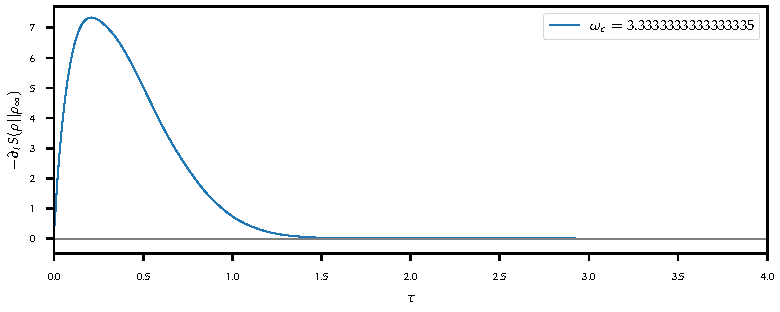
\includegraphics{figs/one_bath_syst/steady_relent}
  \caption{\label{fig:steady_relent} The negative time derivative of
    the relative entropy of system state and the approximate steady
    state (before the interaction is switched off) of the simulations shown in
    \cref{fig:markov_analysis_steady}. The short memory case does not
    violate Spohn's inequality, but the other two cases do. Note
    however, that the \(τ_{\bath}=1\) case has not yet reached a
    steady state and should therefore be treated with care.}
\end{figure}

\Cref{fig:steady_relent} demonstrates that the two simulations with
longer bathe memories are inconsistent with Markovian dynamics, as
their entropy production exhibits strong negativity. The
\(τ_{\bath}=1\) must be taken with care, as the steady state hasn't
been reached yet.

In summary we find that the energy dynamics of system, interaction and
bath depend strongly on the characteristics of the bath.  In the
regime studied, optimizing for fast energy loss of the system favors
longer bath memories, whereas the situation is reversed when longer
coupling times are allowed.

A resonance phenomenon has been observed which is already present in
the weak coupling case. However, here we additionally found a strong
dependence of the dynamics upon the shape of the whole spectral
density.

Note that the short time behaviour discussed here can usually not be
resolved by GKSL dynamics.

\paragraph{Initial Slip}
\begin{figure}[htp]
  \centering
  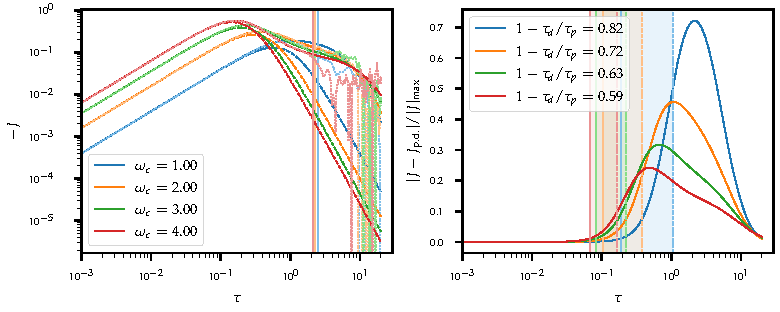
\includegraphics{figs/one_bath_syst/omega_initial_slip}
  \caption{\label{fig:omega_initial_slip} Left panel: The bath energy
    flow of the model \cref{eq:one_qubit_model} for various coupling
    strengths (solid lines) and the pure dephasing flow of
    \cref{sec:pure_deph} (dashed lines). The dotted lines show the
    flow calculated from one trajectory and the vertical lines mark
    the position of the peak of the absolute value of the interaction
    energy. Right panel: The difference of the actual flow \(J\) and
    the pure dephasing flow \(J_\mathrm{p.d.}\). The solid vertical
    lines mark the time \(τ_p\) where the normalized deviation from
    pure dephasing is \(10^{-2}\) and the dashed vertical lines show
    the position of the peak flow at time \(τ_p\). The divergence from
    pure dephasing dynamics occurs before the peak flow and the
    earlier the longer the bath memory. The single trajectory flow
    matches the converged flow for a longer period.}
\end{figure}

As the initial peak in the energy flow is also very prominent in the
simulations in this section we return to
\cref{fig:omega_systematics_system} and compare the dynamics of those
simulations to the pure dephasing case of \cref{sec:pure_deph}.

We see in \cref{fig:omega_initial_slip} that the pure dephasing
dynamics are accurate for very short time scales, but fail to predict
the exact location of the peaks in the bath energy flow. The deviation
from the pure dephasing flow occurs before the peak, where the time
difference between the absolute peak flow and the deviation increases
with increasing bath memory \(\propto 1/ω_c\), as does the magnitude
of the maximal relative deviation. This can be ascertained from the
legend of \cref{fig:omega_initial_slip} where the difference between
deviation and peak time normalized by peak time is given.

We can conclude that for longer bath memories along with weaker
couplings, the role of the system Hamiltonian dynamics in modulating
the flow becomes increasingly important as now the system dynamics
happen on the same time scale as the bath dynamics.

The flow calculated from a single trajectory matches the converged
longer than the pure dephasing flow. For large \(ω_{c}\) the single
trajectory matches until after the peak flow, whereas the deviation
occurs earlier for the \(ω_{c}=1\) case. The stochastic nature of the
single trajectory dynamics seems to become important only after a
finite amount of time, longer than period of pure dephasing
dynamics.

For short times the flow is mainly influenced by the buildup of the
auxiliary states rather than the fluctuations of the stochastic
process, leading to a similar behavior for most trajectories. See
\cref{fig:flow_buildup} an illustration of this phenomenon. This is
most useful, as this period of rapid dynamics must be resolved very
precisely to accurately integrate the flow into the bath energy
change.
\begin{figure}[htp]
  \centering
  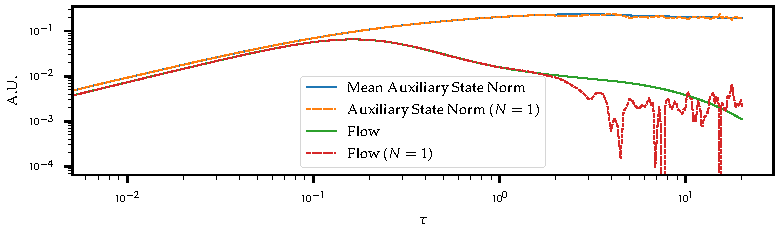
\includegraphics{figs/one_bath_syst/flow_buildup}
  \caption{\label{fig:flow_buildup} The total norm of the first
    auxiliary states and the flow for one trajectory and as a mean
    over all trajectories for the \(ω_{c}=4\) simulation. For short
    times the results for one trajectory match the ensemble means. The
    divergence between one trajectory and the ensemble occurs at
    roughly the same time for the flow and the auxiliary state
    norm. Moreover, flow and mean auxiliary state have the same
    functional form for very short times, apart from a scaling
    factor. The initial dynamics are therefore mainly concerned with
    populating the auxiliary states.}
\end{figure}

\subsection{Varying the Coupling Strength}
\label{sec:one_bathcoup_strength}
\begin{wrapfigure}[17]{O}{0.3\textwidth}
  \centering
  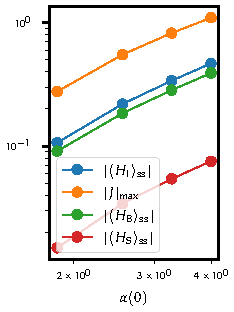
\includegraphics{figs/one_bath_syst/final_states_flows}
  \caption{\label{fig:delta_fs_flow} The absolute difference of the state energies and the
  maximal flows for the simulations in
  \cref{fig:delta_energy_overview} relative to their value at \(α(0)=1.12\).}
\end{wrapfigure}
After having studied the dependence of the bath energy flow for
various cutoff frequencies of the BCF in \cref{sec:one_bath_cutoff},
we now consider the case with fixed cutoff \(ω_c=2\) but varying
coupling strength. The results presented here are mainly a
demonstration of the feasibility of high-consistency simulations for a
range of coupling strengths. We will therefore keep the discussion of
the physical implications relatively short.

The chosen simulation parameters are the same as in
\cref{sec:one_bath_cutoff} and again consistent results have been
obtained as can be gathered from
\cref{fig:delta_interaction_consistency} throughout the whole range of
coupling strengths.
The interaction strength was chosen linearly spaced and the simulation
results are presented in \cref{fig:delta_energy_overview}.

\begin{figure}[htp]
  \centering
  \includegraphics{figs/one_bath_syst/δ_energy_overview}
  \caption{\label{fig:delta_energy_overview} Energy overview for the
    model \cref{eq:one_qubit_model} for various coupling
    strengths. The curves are converged out, and the error funnels are
    not visible.}
\end{figure}
As the shape of the BCF is not altered between the simulations, the
bath energy flows look very similar as do the interaction
energies. The main difference is the magnitude of the interaction
energy. With increased coupling strength there is an increased
interaction energy and an increased flow which leads to faster energy
loss in the system and faster energy gain of the bath. The stronger
the coupling, the more pronounced as the non-monotonicity in time of
the interaction energy, which is reflected in a non-monotonicity in
the bath energy expectation value. The bath energy reaches a maximum
and falls slightly for the strongest coupling simulations. If the
interaction is strong enough, ``backflow'' can occur despite finite
bath correlation times. In \cref{fig:markov_analysis_steady} the bath
memory is long, additionally to a strong coupling so that multiple
oscillations can be seen.

Despite these differences for finite times, the approximate steady
state\footnote{excluding the \(α(0)=0.4\) cases} interaction energies,
maximal flows, system energies and bath energies are almost linearly
dependent on the coupling strength \(α(0)\) in this regime as is
demonstrated in the log-log plot \cref{fig:delta_fs_flow}.

We find that we can control the speed of the energy transfer between
bath and system with the coupling strength at the cost of greater
steady state interaction energy. Were we to turn off the interaction
very fast, we would have to expend this energy in the worst case. On
the other hand, more adiabatic protocol as the one used in
\cref{fig:markov_analysis_steady} would likely be a remedy to this
drawback.

The cooling performance for a coupling that is being turned off at the
end would depend on the concrete protocol as we've seen in
\cref{sec:one_bath_cutoff} and a more detailed study is left to future
work. The interplay between the interaction time-scale mediated by the
coupling strength, the bath memory time and the system dynamics allows
for intricate tuning.

Both the final system and bath energies are increasing with the
coupling strength, compensating for the interaction energy which is
the main mechanism that leads to residual system energy in the steady
state which is further and further away from the ground state, which
would be the steady state of weak coupling dynamics.


\fixme{iftime: re-run with same coupling strength, more cutoff freqs,
  less samples, see, longer times for coupling strengths, more coup}

\section{Some Quantum-Thermodynamic Notions from a Unitary Perspective}
\label{sec:basic_thermo}
After the precision studies of \cref{sec:hopsvsanalyt,sec:prec_sim} we
pause for a brief interlude to introduce some notions that are being
referred to in the subsequent applications of the formalism developed
in \cref{chap:flow}.

The field of quantum thermodynamics is a complex one and we will
restrict the account given here to the minimum required for the
presentation of the subsequent results. A comprehensive account can be
found in
\cite{Binder2018,Kurizki2021Dec,Talkner2020Oct,Vinjanampathy2016Oct}.

Many central questions in thermodynamics are concerned with energy
extraction from macroscopic systems. These questions can be framed in
operational terms that don't require a specific definition of heat and
just relying on energy change in the total system or its
constituents. Energy quantities are now accessible to us in a rather
general settings, making issues related energy extraction a prime
application for our method.

Here, we will focus on the closely related problems. The first is
concerned with how much energy can be extracted through a unitary
transformation from a single infinite thermal bath coupled to an
arbitrary finite dimensional working medium. We call this energy
\emph{ergotropy}\footnote{See \cref{eq:ergo_def} for a more precise definition.}.

The second law of thermodynamics tells us that in this setting no
energy can be extracted in a periodic manner.  It turns out that such
a result can be obtained by studying bounds on the ergotropy of the
system as is done in \cref{sec:ergo_general}. Remarkably these bounds
will turn out to be finite. We will review a general bound for single
bath systems in \cref{sec:ergoonebath} and study an explicit
calculation for a simple case in \cref{sec:explicitergo}. The latter
study will elucidate under which conditions we may expect the bound to
be tight.

The second problem is a generalization of the above considerations to
systems coupled to multiple baths of different temperature. Here,
naturally, the ergotropy is generally not bounded. However, there is a
limit to how efficiently energy can be extracted. To quantify
efficiency one has to introduce a notion of thermodynamic
cost. Traditionally this is the entropy production or the amount of
``waste heat'' that is being shed into the cold reservoir instead of
being extracted as work. Both quantities require a proper definition,
which can usually be given, but is not unique due to the issue of
finite interaction energy\footnote{See the discussion in
  \cref{chap:intro}.}.

Nevertheless, when the system is periodically modulated so that the
interaction is turned off at some point in each cycle, we can clearly
divide system and bath energies. In this case it becomes clear, that
we can define the efficiency for a system with a hot and a cold bath as
\begin{equation}
  \label{eq:efficiency_definition}
  η = \frac{Δ\ev{H_{\bath}}_{\mathrm{cyc},c}}{Δ\ev{H}_{\mathrm{cyc}}},
\end{equation}
where \(Δ\ev{H_{\bath}}_{\mathrm{cyc},c}\) is the cold bath energy change
over one cycle and \({Δ\ev{H}_{\mathrm{cyc}}}\) is the total energy
change over one cycle.

In \cref{sec:operational_thermo} a Gibbs like inequality for an
arbitrary number of baths is derived, further strengthening the
importance of those notions. The left hand side of this inequality can
be associated with a thermodynamic cost that should be minimized for
optimal efficiency.


\subsection{The Ergotropy of Open Quantum Systems with a single Bath}
\label{sec:ergo_general}
\begin{itemize}
\item introduce ergotropy and passivity as basis for the rest
\end{itemize}
The ergotropy of a quantum system is defined\fixme{mention paper that
  uses ergo for heat}
as~\cite{Binder2018}
\begin{equation}
  \label{eq:ergo_def}
  \ergo{ρ} = \max_{U\,\text{unitary}}\tr[\qty(ρ - UρU^\dag) H],
\end{equation}
which is the maximal energy that can be extracted from a system through
cyclic modulation of the Hamiltonian \(H\). A state is called passive
iff the maximizing \(U\) \cref{eq:ergo_def} is the identity \(\id\).

A passive state \(ρ_P\) is always diagonal in the eigenbasis of \(H\) and its
eigenvalues satisfy the following ordering condition~\cite{Lenard1978Dec}
\begin{equation}
  \label{eq:passive_diag}
  ρ_{p}=∑_{j=1}^{n} \lambda_{j}|j\rangle\langle j|, \quad E_{j} \leq E_{j+1}, \quad \lambda_{j+1} \leq \lambda_{j},
\end{equation}
where \(n<∞\) is the Hilbert space dimension. This condition is both
necessary and sufficient. Examples of passive states are the state of
the micro-canonical ensemble or a Gibbs state. Gibbs are further
distinguished by additional features as described
in~\cite{Lenard1978Dec}, which can be connected to formulations of the
zeroth and second laws of thermodynamics.

One of these properties is complete passivity. Completely passive
states remain passive under the transformation \(ρ\to\otimes^Nρ\) (and
an \(N\)-fold sum of the Hamiltonian) for finite \(N\). Therefore no
energy can be extracted from multiple identical systems at the same
temperature. For finite dimensional systems, the complete passivity
implies the form of the Gibbs state. The open-systems case differs as
here a ``small'' system is coupled to a bath of infinite size. If the
system state is not a Gibbs state, the whole system becomes
non-passive, even if the system state is passive with respect to the
system Hamiltonian\footnote{for example being the ground state}.

For systems of infinite size, states fulfilling the
Kubo–Martin–Schwinger (KMS) condition have been proposed as the
generalizations of Gibbs states, having similar properties as
Gibbs states. Under some conditions passivity implies the KMS
condition. These conditions are related to the fact that KMS states
are not necessarily unique~\cite{Binder2018,Pusz1978Oct}.

The KMS condition is stated for two arbitrary observables \(A,B\) and
\(F_{AB}(t)=\tr[ρ_βA(t)B(0)]\) (Heisenberg picture,
\(A(t)=\eu^{\iu H t}H\eu^{-\iu H t}\)) as
\begin{equation}
  \label{eq:kmscond}
  F_{AB}(-t) = F_{BA}(t-\iu β)
\end{equation}
by virtue of analytic continuation.

For two initially uncorrelated KMS states, of different
temperature, the Carnot efficiency bound can be
proven~\cite{Pusz1978Oct}.

A simple application of ergotropy is an explanation for quantum
friction. The buildup of coherence\footnote{Meaning a state which is
  non-diagonal in the energy basis.} in a quantum system makes the
state non-passive and thus requires additional energy which cannot be
extracted by modulating of the energy level gaps of the
system\footnote{This is the usual mechanism of energy extraction in a
  quantum Otto cycle~\cite{Geva1992Feb}.}~\cite{Kurizki2021Dec}.  The
reduction of efficiency in through quantum coherence general has been
termed quantum friction. However, the occurrence of coherence does not
have to lead to a reduction in efficiency\fixme{do more research on
  that.refer to simulations}, if a diagonal state is restored \footnote{Shortcuts to
  adiabaticity, see for example~\cite{Chen2010Feb}.}.

\subsection{The Ergotropy of Finite Systems Coupled to a Thermal Bath}
\label{sec:ergoonebath}
\begin{itemize}
\item thermal states are somewhat special (as seen above)
\item for thermodynamic consistency: we want to find a general bound
  on ergotropy that may be valid also in the infinite dimensional case
\item great news: model independent and gives meaning to temperature!
\end{itemize}
Let us consider models with the Hamiltonians
\begin{equation}
  \label{eq:simple_bath_models}
  H = \id_\sys\otimes H_\bath + H_\sys\otimes \id_\bath,
\end{equation}
where the system \(\sys\) is finite dimensional and \(H_\bath\) may
chosen arbitrarily. Let the initial state of the system be
\begin{equation}
  \label{eq:simple_initial_state}
  ρ=ρ_\sys\otimes τ_β,
\end{equation}
where \(τ_β=\eu^{-β H_\bath}/Z\) and \(ρ_\sys\) is arbitrary.

An interesting question is whether the ergotropy of such a state is
finite. This amounts to the formulation of the second law: ``No energy
may be extracted from a single bath in a cyclical manner''.
For systems obeying GKSL dynamics connected to a KMS state heat bath,
thermodynamic laws can be derived in certain situations\footnote{very
  slow or very fast modulation of the system
  hamiltonian}\cite{Binder2018}, which imply the answer ``yes'' for the
above questions. In the non-Markovian case, those arguments do not
hold anymore.

For finite dimensional baths, we always have finite ergotropies, as
their Hamiltonians are bounded. In the infinite dimensional case, we
may expect that the ergotropy is still finite for some models, as long
as the energies of the thermal states for those models is finite. This
assumption breaks down when we consider infinite baths, whose thermal
energy is unbounded even for finite temperatures.

Nevertheless, \fixme{graphics} the ergotropy appears to be
bounded. Further, the system as if it was in a passive state as soon
as the limit cycle is reached. In fact, there is a simple and general
argument that provides and upper bound on the ergotropy of states of
the form~\cref{eq:simple_initial_state} based on the special form of
Gibbs states and relative entropy. The latter quantity allows the
application of quantum informational tools, even in the presence of
infinite baths if we are careful in taking limits.

The following is adapted
from~\cite{Biswas2022May,Alicki2013Apr,Lobejko2021Feb} and we limit
ourselves to finite dimensional problems for now.  As unitary
transformations leave the entropy invariant
(\(\tr[ρ\ln(ρ)] = \tr[ρ_P\ln(ρ_P)]\)), we have for an arbitrary
\(β > 0\) and \(ρ_β=\exp(-βH)/Z\)
\begin{align}
    \ergo{ρ} &= E(ρ) - E(ρ_P) = \tr[(ρ-ρ_P) H]\nonumber\\
             &= -\frac{1}{β}\tr[(ρ-ρ_P)
               \qty(\ln(ρ_β) + \ln(Z))] \nonumber\\
             &= -\frac{1}{β}\tr[(ρ-ρ_P) \ln(ρ_β)] =
               -\frac{1}{β}\tr[(ρ-ρ_P) \qty(\ln(ρ_β))]\nonumber\\
             &=\frac{1}{β}\qty[\tr[ρ(\ln(ρ) - \ln(ρ_β))] -
               \tr[ρ_P(\ln(ρ_p) - \ln(ρ_β))]]\nonumber\\
             &\equiv\frac{1}{β}\qty[\qrelent{ρ}{ρ_β} - \qrelent{ρ_P}{ρ_β}]\label{eq:ergo_entro},
\end{align}
where we have used \(\tr[ρ]=\tr[ρ_P]=1\).

The relative entropies
appearing in \cref{eq:ergo_entro} are always finite, as \(ρ\) is
finite-dimensional and \(ρ_β\) has full rank.  As energy is minimized
by a Gibbs state when keeping the entropy fixed, we find an upper
bound on the ergotropy by replacing \(ρ_P\to ρ_{β^\ast}\) in
\cref{eq:ergo_entro} where
\(S(ρ_{β^\ast})=S(ρ)\)~\cite{Alicki2013Apr}.

By choosing the temperature in \cref{eq:ergo_entro} accordingly, we
arrive at
\begin{equation}
  \label{eq:ergo_bound_single}
  \ergo{ρ} \leq \frac{1}{β^\ast}\qrelent{ρ}{ρ_{β^\ast}}.
\end{equation}
This bound can be saturated for states which are a permutation of a
thermal state, as their corresponding passive states is the thermal
state.

For our setting in
\cref{eq:simple_bath_models,eq:simple_initial_state} we find a still
better way to bound the ergotropy and fix the
temperature~\cite{Lobejko2021Feb}. Substituting \(ρ\to ρ \otimes τ_β\)
in \cref{eq:ergo_entro} we obtain
\begin{equation}
  \label{eq:thermo_ergo_bound}
  \begin{aligned}
  \ergo{ρ\otimes τ_β} &= \frac{1}{β}
  \qty[\qrelent{ρ\otimes τ_β}{ρ_β\otimes τ_β} - \qrelent{(ρ\otimes
                        τ_β)_P}{ρ_β\otimes τ_β}]\\
    &=\frac{1}{β}
  \qty[\qrelent{ρ}{ρ_β} - \qrelent{(ρ\otimes τ_β)_P}{ρ_β\otimes
      τ_β}] \leq \frac{1}{β} \qrelent{ρ}{ρ_β}.
  \end{aligned}
\end{equation}

Remarkably, the bound \cref{eq:thermo_ergo_bound} only depends on the
system state and ``inherits'' the temperature of the bath. For any
\(\dim[τ_β] = N\gg 1\) the bound stays valid. It is therefore
reasonable to expected that it is also valid for an infinite bath. On
the basis of physical intuition, a very large but finitely sized bath
may be an arbitrarily good substitute for a continuous one. One might
even argue, that the continuous bath is a mathematically convenient
construct and the finite bath is the physical one.  The objection to
taking the limit outright is that the state \(τ_β\) does not exist as
trace class operator for an infinite bath.

Interestingly, a saturation of \cref{eq:thermo_ergo_bound} is achieved
in~\cite{Skrzypczyk2014Jun} with a continuous qubit
bath. In~\cite{Lobejko2021Feb} a more generic argument is made in a
similar setting. Both propose concrete protocols within the bounds of
thermal operations and by considering explicit work reservoirs.

For the term \(\qrelent{(ρ\otimes τ_β)_P}{ρ_β\otimes τ_β}\) to vanish
in \cref{eq:thermo_ergo_bound}, the state bath and system should be as
close to the product thermal state as possible and so the bath state
should not change too much. This is achievable with a continuous
infinite size bath.  As \(ρ_β\otimes τ_β\) is the steady state of GKSL
dynamics (without modulation) under mild
assumptions~\cite{Binder2018}, it can be said that in this case
ergotropy is being lost.

A corollary of \cref{eq:thermo_ergo_bound} is the Clausius form of the
second law. By setting the system Hamiltonian to \(α \id\) in the
above discussion the ergotropy becomes the change of bath energy
\begin{equation}
  \label{eq:ergo_bath_change}
  \begin{aligned}
    \ergo{ρ} &= \max_{U\,\text{unitary}}\tr[\qty(ρ - UρU^\dag)
               (α\id\otimes H_\bath)] \\
             &=\max_{U\,\text{unitary}}\tr_\bath[\qty(\tr_\sys[ρ-UρU^\dag])
               H_\bath]\\
             &\equiv\max_{U\,\text{unitary}}ΔE_\bath\leq \frac{1}{β}\qrelent{ρ}{\frac{\id_N}{N}},
  \end{aligned}
\end{equation}
where \(N\) is the system dimension. No finite amount of energy may
therefore be extracted from the bath in a periodic manner. If it were
possible to extract a constant positive amount of energy from the bath
per cycle, \cref{eq:ergo_bath_change} would be breached in finite
time.


\subsection{The Ergotropy of a Two
  Level System and a Bath of Identical Oscillators}
\label{sec:explicitergo}
\begin{itemize}
\item as an illustrative example: calculate ergotropy for a concrete
  model
\item can show us how good the bound derived earlier is and whether it
  holds for these infinite dimensional systems
\end{itemize}

Here, we explicitly calculate the ergotropy of a finite dimensional
system connected to a bath of identical oscillators. Throughout we
will set the zero-point energy of the oscillators to zero, meaning
that \(H=ωa^\dag a\) for a single harmonic oscillator with the usual
annihilation operator \(a\).


Let us choose \(H_S=α\id_N\)  for simplicity,
where \(α\) is an arbitrary energy scale. The ergotropy is then equal
to the maximal energy reduction of the bath under arbitrary cyclic
modulation.

The bound \cref{eq:thermo_ergo_bound} further simplifies to
\begin{equation}
  \label{eq:thermo_ergo_bound_specific}
  \ergo{ρ\otimes τ_β} \leq \frac{1}{β} \qty[\ln(N) - S(ρ)],
\end{equation}
where \(S(ρ)=-\tr[ρ\ln(ρ)]\).  For a pure state
\cref{eq:thermo_ergo_bound_specific} is maximal and we therefore choose
\(ρ=\ketbra{0}\) as an arbitrary pure state.

If we take the system to be a qubit, the right hand side of
\cref{eq:thermo_ergo_bound_specific} is the Landauer bound
\(β^{-1}\ln2\). Therefore, up saturation of the bound
\cref{eq:thermo_ergo_bound_specific} we can extract enough energy from
the bath to erase one bit in a system of the same temperature as the
bath. Indeed, owing to \cref{eq:thermo_ergo_bound_specific} the closer
the qubit state is to the infinite temperature (erased) state the more
certain we are, that we have extracted the maximum energy out of the
bath.


\paragraph{One Oscillator}
As a demonstration of the general program, let us first discuss the
ergotropy of a single harmonic oscillator with frequency \(ω\) as a
bath.  The initial state is given by
\begin{equation}
  \label{eq:onehoinit}
  ρ_{0} = ∑_{n=0}^{∞} \underbrace{Z^{-1}\eu^{-βωn}}_{λ_{0,n}} \ketbra{{0,n}},
\end{equation}
where \(Z=Z_{1}=\frac{1}{1-\eu^{-βω}}\) is the partition sum of one
bosonic mode with frequency \(ω\).

In contrast to the state characterized by \cref{eq:passive_diag} we
only fill every second level with \cref{eq:onehoinit}. To construct a
corresponding passive state\footnote{Due to the degeneracy of the
  system Hamiltonian, the passive state is not unique.} we have to
construct a sequence \(λ_{i},\, i \in \NN_{0}\) out of the weights
\(λ_{0,n}\) such that \(λ_{i}\geq λ_{j}\) for \(i\leq j\) and a
sequence of states \(\ket{j}\) so that for \(\ev{H}{j} = E_{j}\) we
have \(E_{i}\leq E_{j}\) for \(i\leq j\). The passive state and its
corresponding energy is then
\begin{equation}
  \label{eq:specific_passive_state}
  \begin{aligned}
    ρ_{p} &= ∑_{i} λ_{i} \dyad{i} & E_{p} &= ∑_{i} λ_{i}E_{i}.
  \end{aligned}
\end{equation}

In the present case, this is easily done by defining \(λ_{i}=λ_{0,i}\)
and
\begin{equation}
  \label{eq:state_enumeration_single}
  \ket{i} =
  \begin{cases}
    \ket{0, i/2} & i\text{ even} \\
    \ket{1, (i - 1) / 2} & i\text{ odd}. \\
  \end{cases}
\end{equation}

Thus, we find a passive state
\begin{equation}
  \label{eq:one_ho_pass}
  ρ_{p} = \frac{1}{Z} \qty[∑_{i} \eu^{-2i βω} \ketbra{0, i} +
  \eu^{-(2i + 1) βω} \ketbra{1, i}].
\end{equation}

The corresponding energy difference \(\ev{H (ρ_{0} - ρ_{p})}\) works
out to be
\begin{equation}
  \label{eq:one_ho_ergo}
  \mathcal{W} = ω\qty(\frac{1}{\eu^{βω} - 1} - \frac{1}{\eu^{2βω} - 1}) = ω \frac{\eu^{-β ω} - \eu^{-2 β ω}}{1-\eu^{-β
      ω}-\eu^{-2 β ω} + \eu^{-3 β ω}} \xrightarrow{βω
    \rightarrow ∞} \frac{ω}{\eu^{βω} - 1}.
\end{equation}

For low temperatures or large frequencies, the ergotropy of the
oscillator is just its mean thermal energy \(ω\bose(ωβ)\). In the
opposite limit we find
\(\mathcal{W} = \frac{1}{7β}< β^{-1}\ln(2)\)\fixme{check calculations
  :P}.

\paragraph{Many Oscillators}
For the case of \(N>1\) oscillators with frequency \(ω\) the initial
state is
\begin{equation}
  \label{eq:manyhoinit}
  ρ_{0} = ∑_{\vb{n}\in\ZZ_{0}^{n}} \underbrace{Z^{-1}\eu^{-βω\abs{\vb{n}}}}_{λ_{0,\vb{n}}} \ketbra{{0,\vb{n}}},
\end{equation}
with the \(n_{i}=(\vb{n})_{i}\) labeling the state of the \(i\)th
oscillator and \(\abs{\vb{n}}=∑_{i=1}^{N}n_{i}\) and \(Z=Z_{1}^{N}\).

In this case we again call the ordered sequence of weights \(λ_{i}\),
but its construction is somewhat more complicated and we will refrain
from doing so here explicitly.
Instead we take an enumeration of state labels
\(\{\vb{n}^{i}\}_{i\in\NN_{0}}\) such that
\(i<j \implies m_{i} \leq m_{j}\) with
\(m_{i}\equiv\abs{\vb{n}^{i}}\). The energies of the states
\(\ket{k,\vb{n}^{i}}\) evaluate to \(E_{k, i} = ω m_{i}\) and the
weights to \(λ_{0,i}=Z^{-1}\eu^{-βω m_{i}},\,λ_{1,i}=0\).

The required enumeration of states and energies is then
\begin{equation}
  \label{eq:many_enum}
  \begin{aligned}
  \ket{i} &=
  \begin{cases}
    \ket{0, m_{i/2}} & i\text{ even} \\
    \ket{1, m_{(i-1)/2}} & i\text{ odd}
  \end{cases},
    & E_{i} &= ω m_{\lfloor{i/2}\rfloor}
  \end{aligned}
\end{equation}
and the enumeration of weights is \(λ_{i} = λ_{0,i} =Z^{-1}\eu^{-βω m_{i}}\).


The corresponding passive state energy will be
\begin{equation}
  \label{eq:many_ho_pass}
  E_{p} = \frac{ω}{Z} ∑_{i=0}^{∞} m_{i} \pqty{\eu^{-ωβ m_{2i}} + \eu^{-ωβ m_{2i+1}}}.
\end{equation}

For each value of \(m\) of \(\qty{m_{k}}\) there are
\(G_{m}^{N} = \binom{N+m-1}{N-1}\) sequence elements \(m_{i}\) with
\(m_{i}=m\).  We define the sequence \(\qty{x_{m}}_{m\in\NN_{0}}\) so
that \(x_{m}=G^{N+1}_{m}=\binom{N+m}{m}\) denotes the index \(i\)
until which \(m_{i}\) has the value \(m\). Likewise
\(\qty{y_{m}}_{m\in\NN_{0}}\) is defined so that
\(y_{m}=\big\lceil G^{N+1}_{m}/2\big\rceil\) denotes the index \(i\)
until which \(m_{2i}\) has the value \(m\). When using the floor
instead of ceil in the definition of \(y_{m}\) we find that this
sequence \(\qty{z_{m}}_{m\in\NN_{0}}\) fulfills the same purpose but
for \(m_{2i+1}\).

Now, let
\begin{equation}
  \label{eq:deltas}
  \begin{aligned}
    Δ^{e}_{m,m} &= y_{m}-x_{m-1}
                  =\left\lceil\frac{G^{N+1}_{m}}{2}\right\rceil -
                  G^{N+1}_{m-1} & Δ^{e}_{m,m+1} &= x_{m}-y_{m}
                  =G^{N+1}_{m} - \left\lceil\frac{G^{N+1}_{m}}{2}\right\rceil\\
  Δ^{o}_{m,m} &= z_{m}-x_{m-1}
                  =\left\lfloor\frac{G^{N+1}_{m}}{2}\right\rfloor -
                  G^{N+1}_{m-1} & Δ^{o}_{m,m+1} &= x_{m}-z_{m}
                  =G^{N+1}_{m} - \left\lfloor\frac{G^{N+1}_{m}}{2}\right\rfloor.
  \end{aligned}
\end{equation}

The \(Δ^{e}_{m,k}\) denotes the number of indices \(i\) where
\(m_{i}=m\) and \(m_{2i}=k\) and the \(Δ^{e}_{m,k}\) have the same
function, but for \(m_{2i+1}\).
The equations \cref{eq:deltas} lists explicit formulas only for the
case, where the difference is at most one, but this is sufficient for
the estimate we will discuss now.

We find
\begin{equation}
  \label{eq:manhoergoestimate}
  \begin{aligned}
    E_{p} &\geq \frac{ω}{Z} ∑_{m=1}^{∞} m \bqty{\eu^{-m
            ωβ}\pqty{Δ^{o}_{m,m} + Δ^{e}_{m,m}} + \eu^{-(m+1)
            ωβ}\pqty{Δ^{o}_{m,m+1} + Δ^{e}_{m,m+1}}} \\
          &= \frac{ω}{Z} ∑_{m=1}^{∞} m\eu^{-m
            ωβ} \bqty{G^{N+1}_{m} - 2 G^{N+1}_{m-1} +
            G^{N+1}_{m}\eu^{-ωβ}}\\
          &= \frac{ω}{Z} ∑_{m=1}^{∞} m\eu^{-m
            ωβ} \bqty{G^{N}_{m} - G^{N+1}_{m-1} + G^{N+1}_{m}\eu^{-ωβ}},
  \end{aligned}
\end{equation}
where we have used that all summands are nonnegative and we could
therefore obtain a lower bound on the passive energy by dropping all
terms where the difference between \(m_{i}\) and \(m_{2i}\,,m_{2i+1}\)
is greater than one. The terms for which this is true will have large
values of \(m\) and will further be suppressed by a factor of
\(\eu^{-kωβ}\) (\(k\geq 2\)) so one might expect this bound to be
tight for large \(ω\) and large \(N\).

We can evaluate \cref{eq:manhoergoestimate} further by noting
\begin{equation}
  \label{eq:many_ho_orig_energy}
  E_{0} = \tr[ρ_{0}H]
  = \frac{1}{Z} ∑_{\vb{n}\in\NN_{0}^{N}} ω\abs{\vb{n}}
  \eu^{-\abs{\vb{n}}ωβ}
  = \frac{ω}{Z} ∑_{m=1}^{∞} m G^{N}_{m}\eu^{-mωβ}
\end{equation}
and also
\begin{equation}
  \label{eq:manhoergoestimate_further}
  \begin{aligned}
    ∑_{m=1}^{∞} m\eu^{-m
    ωβ} &\bqty{- G^{N+1}_{m-1} + G^{N+1}_{m}\eu^{-ωβ}} \\
        &=
          -∑_{m=0}^{∞} (m+1)\eu^{-(m+1)
          ωβ} G^{N+1}_{m}  + ∑_{m=1}^{∞} m
          G^{N+1}_{m}\eu^{-(m+1)ωβ}\\
        &= -∑_{m=0}^{∞} (m+1)\eu^{-(m+1)
          ωβ} G^{N+1}_{m}  + ∑_{m=0}^{∞} m
          G^{N+1}_{m}\eu^{-(m+1)ωβ} \\
        &= -∑_{m=0}^{∞} G_{m}^{N+1}\eu^{-(m+1)ωβ} =-\eu^{-ωβ}
          ∑_{\vb{n}\in\NN_{0}^{N+1}}\eu^{-\abs{\vb{n}} ωβ}\\
        &= -\eu^{-ωβ} Z_{N+1} = -\eu^{-ωβ} Z_{1}^{N+1},
  \end{aligned}
\end{equation}
where we shifted indices and used some properties of the
\(G_{m}^{N}\).

Finally, we arrive at
\begin{equation}
  \label{eq:many_ho_ergo_bound_prelim}
  E_{p} \geq E_{0} - ω \frac{Z_{1}^{N+1}}{Z_{1}^{N}} \eu^{-ωβ} = E_{0} - ω
  \bose(ωβ),
\end{equation}
which yields
\begin{equation}
  \label{eq:many_ho_ergo_bound}
  \mathcal{W} \leq ω \bose(ωβ) = E_{1}.
\end{equation}

So the ergotropy of \(N\) oscillators is bounded by the thermal energy
of a single oscillator. This bound converges to the exact ergotropy as
\(ωβ\rightarrow ∞\) as the terms left out in
\cref{eq:manhoergoestimate} do not contribute in this limit.

For \(ωβ\ll 1\) we neglect the lower values of \(m\) in
\cref{eq:many_ho_pass} and estimate for \(N\gg 1\) and \(m\gg 1\)
\begin{equation}
  \label{eq:high_t_estimate_ergo}
  i \sim G_{m_{i}}^{N+1} = \frac{m+N}{N!m!}
  = \frac{(m+N)(m+N-1)\ldots (m+1)}{N!} =\frac{m_{i}^{N}}{N!} + O(m^{N-1})
\end{equation}
yielding
\begin{equation}
  \label{eq:m_of_i}
  m_{i}\sim \pqty{N!i}^{\frac{1}{N}} \implies m_{2i} \sim
  2^{\frac{1}{N}}m_{i} \sim m_{2i+1}.
\end{equation}

Using this, \cref{eq:many_ho_pass} becomes\fixme{I'm still amazed that
this works.}
\begin{equation}
  \label{eq:passive_e_many_high_T}
  E_{p} \sim \frac{ω}{Z} ∑_{i=0}^{∞} 2 m_{i} \eu^{-ωβ 2^{\frac{1}{N}} m_{i}}
  = ω N \bose(ωβ 2^{\frac{1}{N}}),
\end{equation}
where \(Z=2 ∑_{i=0}^{∞}\eu^{-ωβ 2^{\frac{1}{N}} m_{i}}\) was used for
consistency.

Finally we can use \cref{eq:passive_e_many_high_T} to estimate the
ergotropy
\begin{equation}
  \label{eq:ergo_esti_high_t}
  \mathcal{W} = ω N\pqty{\frac{1}{\eu^{ωβ} - 1} -
    \frac{1}{\eu^{2^{\frac{1}{N}}ωβ} - 1}} \xrightarrow{N\rightarrow
    ∞} ω^{2}β \ln(2) \frac{\eu^{βω}}{\pqty{\eu^{ωβ} -
      1}^{2}}.
\end{equation}

In the limit \(βω\ll 1 \iff ω \ll T\) (continous bath) we further find
\(\mathcal{W} \rightarrow β^{-1} \ln(2)\) which saturates the bound
\cref{eq:thermo_ergo_bound_specific}. This is in concert with
\cite{Skrzypczyk2014Jun,Lobejko2021Feb} where it was found, that an
infinite continous bath is required for the saturation of the bound.

A similar scheme to the one used in \cref{eq:manhoergoestimate} can be
employed numerically to compute the exact ergotropy efficiently and to verify our
findings as has been done in.
\begin{figure}[htp]
  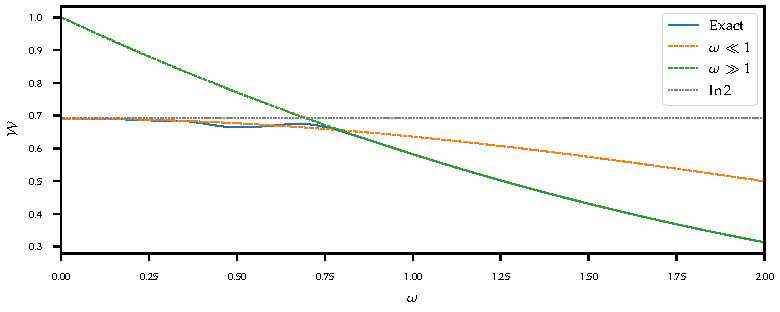
\includegraphics{figs/ergo_calc/ergo_numeric}
  \caption{\label{fig:numeric_n_ho_ergo} Numerical evaluation of
    \cref{eq:many_ho_pass} and the estimates
    \cref{eq:many_ho_ergo_bound,eq:ergo_esti_high_t} for \(N=110\)
    and \(β=1\). Good agreement can be found and the bound
    \(β^{-1}\ln2\) is approximately saturated.}
\end{figure}

In conclusion, we have found an upper bound
\cref{eq:many_ho_ergo_bound} for and a high temperature estimate
\cref{eq:ergo_esti_high_t} of the ergotropy to \(N\) oscillators in a
thermal state and a two level system in a pure state. The bound
\cref{eq:thermo_ergo_bound_specific} on ergtropy is still valid and
also tightest in the infinite bath case with vanishing level distance
\(ω\to 0\). We find that in order to saturate the bound, a bath of
infinite size and vanishing level spacing is required. These
conditions are fulfilled for the baths usually considered in open
quantum systems, where a continuum of frequencies are present instead
of a single, very degenerate one.

Even for finitely many oscillator the ergtropy bound can be approached
rather closely for finite \(ω\) as can be seen in
\cref{fig:numeric_n_ho_ergo_nonmon}. Remarkably, the ergotropy becomes
a non-monotonous function of level spacing \(ω\) for larger \(N\)
while always increasing with \(N\). Also, for large \(N\) the
transition into the region where the estimate upper bound
\cref{eq:thermo_ergo_bound} is tight is very close to the crossing
point of this bound with the \(ω\ll 1\) estimate and the bound is very
tight as may be expected, because the error one makes in
\cref{eq:manhoergoestimate} becomes negligible in the case \(N\gg 1\).
\begin{figure}[htp]
  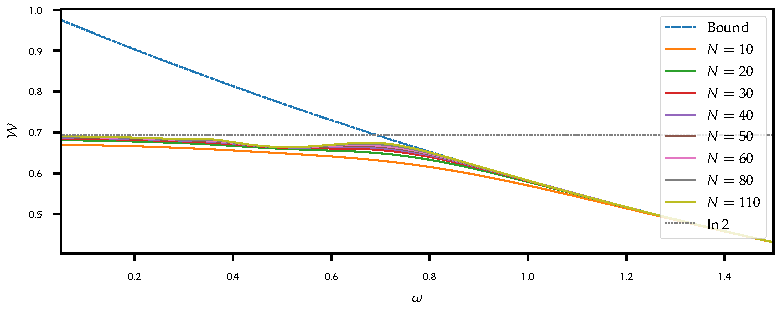
\includegraphics{figs/ergo_calc/ergo_nonmonotonic}
  \caption{\label{fig:numeric_n_ho_ergo_nonmon} Numerical evaluation of
    \cref{eq:many_ho_pass} for different \(N\) and \(β=1\).}
\end{figure}


\subsection{A bound on the Energy Change of Multiple Baths in the
  Periodic Steady State}
\label{sec:operational_thermo}
\begin{itemize}
\item for multiple baths of differing temperatures: previous
  discussions not applicable
\item nevertheless, there is a limit on the combined energy change of
  the baths in the PSS
\item a gibbs like inequality is derived, the left-hand-side may be
  interpreted as thermodynamic cost, maybe input for future optimizations
\end{itemize}
As in the single bath case, some statement about the amount of energy
that can be expected to be extracted in a cyclic manner. An argument
based on entropy may be made for the periodic steady state as was
shown in~\cite{Kato2016Dec} and is reproduced here. We will find the
Clausius form of the second law.

We consider the situation given by the Hamiltonian for a system
coupled to multiple baths under periodic driving
\begin{equation}
  \label{eq:katoineqsys}
  H(t) = H_\sys(t) + ∑_i \qty(H_\bath^i + H_\inter^i(t)).
\end{equation}
Here, \(H_\sys(t)\) is the system Hamiltonian, \(H_\bath^i\) is the
Hamiltonian of the \(i\)-th bath and \(H_\inter^i(t)\) is the coupling
to the same. Again, the bath must be treated as finite during the
derivation.

The von Neumann entropy \(S(t)=-\tr[ρ\ln ρ]\) of the global state whose
evolution is generated by \cref{eq:katoineqsys} is
constant. Additionally \(S\) is sub-additive meaning
\begin{equation}
  \label{eq:subadd}
  S(t) \leq -\tr[ρ_\sys(t)\ln ρ_\sys(t)] - ∑_i\tr[ρ_{\bath^i}(t)\ln
  ρ_{\bath^i}(t)] \equiv S_\sys(t) + ∑_iS_{\bath^i}(t),
\end{equation}
where \(ρ_{\sys}(t)=\tr_{\bigotimes_i{\bath^i}}[ρ(t)]\) and
\(ρ_{\bath^i}=\tr_{\sys\bigotimes_{j\neq i}{\bath^j}}[ρ(t)]\) are the
marginal states of system and the \(i\)th bath respectively. Note that
the marginal entropies \(S_{\sys},\,S_{\bath}\) are generally
\emph{not} constant in time.

This implies for \(ΔS_\sys(t)\equiv S_\sys(t) - S_\sys(0)\) and
\(ΔS_{\bath^i}(t)\equiv S_{\bath^i}(t) - S_{\bath^i}(0)\)
\begin{equation}
  \label{eq:deltagreat}
  ΔS_\sys(t) + ∑_i ΔS_{\bath^i}(t) \geq 0.
\end{equation}

The von Neumann entropy of a single bath can be expressed as
\begin{equation}
  \label{eq:bathentro}
  \begin{aligned}
  S_{\bath^i}(t) &=-\tr[ρ_{\bath^i}(t)\ln ρ_{\bath^i}^β] -
                   \qty(\tr[ρ_{\bath^i}\ln ρ_{\bath^i}(t)] -
                   \tr[ρ_{\bath^i}(t)\ln ρ_{\bath^i}^β])\\
                 &= β E_{\bath^i}(t) - βF_{\bath^i} - \qrelent{ρ_{\bath^i}(t)}{ρ_{\bath^i}^β},
  \end{aligned}
\end{equation}
where
\(E_{\bath^i}(t)=\tr[ρ_{\bath^i}(t)H_{\bath^i}]=\tr[ρ(t)(H_{\bath^i}\otimes
\id)]\), \(ρ_{\bath^i}^β=\exp(-β H_{\bath^i})/Z\) and
\(F_{\bath^i}=-\ln(Z_{\bath^i})/β\) is the equilibrium free energy of
the bath at (as yet undetermined) inverse temperature \(β\).
The result \cref{eq:bathentro} implies
\begin{equation}
  \label{eq:bathenergychange}
  ΔS_{\bath^i}(t) = β_i ΔE_{\bath^i}(t) -
  \qrelent{ρ_{\bath^i}(t)}{ρ_{\bath^i}^{β_i}} \leq β_i ΔE_{\bath^i}(t).
\end{equation}
Note that \(β_i\) is now being fixed through
\(\qrelent{ρ_{\bath^i}(0)}{ρ_{\bath^i}^{β_i}}\Leftrightarrow
{ρ_{\bath^i}(0)}={ρ_{\bath^i}^{β_i}}\).

Combining \cref{eq:bathenergychange,{eq:deltagreat}} yields
\begin{equation}
  \label{eq:bathenergyandsystementro}
  ΔS_\sys(t) + ∑_iβ_i ΔE_{\bath^i}(t) \geq 0.
\end{equation}
This inequality only contains quantities that can be expected to be
finite, even in the limit of infinite baths.

As in \cref{sec:ergoonebath} we now demand periodic driving, that is
\(H(t+τ) = H(t)\) for some \(τ\geq 0\). Now we \emph{Assume} that the
system enters a periodic steady state after the time \(n_0τ\) for some
\(n_0\in\NN\) so that \(ρ_\sys((n + n_0)τ)= ρ_\sys(n_0τ)\) for all
\(n\in\NN\). This assumption is linked to the notion of a ``finite
memory'' of the baths. In the same spirit, we \emph{assume} that the
energy change of each bath
\(ΔE_{\bath^i}^\cyc =ΔE_{\bath^i}((n+1)τ)-ΔE_{\bath^i}(nτ) =
E_{\bath^i}((n+1)τ)-E_{\bath^i}(nτ)\) is constant once the system is
in the periodic steady state. This behavior, at least on the system
level, is suggested by the NMQSD equation \cref{{eq:multinmqsd}}.

As the system entropy does not change over a cycle
\(ΔS_\sys^\cyc = ΔS_\sys(τ (n+n_0)) - ΔS_\sys(τ n_0)=S_\sys(τ (n+n_0)) - S_\sys(τ
n_0)=0\) vanishes we have
\begin{equation}
  \label{eq:secondlaw_cyclic}
  ∑_iβ_i ΔE_{\bath^i}^\cyc \geq 0,
\end{equation}
as otherwise the inequality \cref{eq:bathenergyandsystementro} would
be violated in finite time.

The left hand side could be called ``bath entropy production'' as is
motivated in \cite{Riechers2021Apr}, where heat is identified with
\(ΔE_{\bath^i}\). There also an entropy production bound that takes
into account system and bath is being considered and brought into
connection with information-theoretic quantities.

If one defines heat as is done in
\cite{Kato2016Dec,Riechers2021Apr,Strasberg2021Aug} as the change of
bath energy, \cref{eq:secondlaw_cyclic} amounts to the Clausius form
of the second law. This definition of heat is corroborated
in~\cite{Esposito2015Dec} where it is shown\footnote{for fermionic
  baths} that a definition of heat involving any nonzero fraction of
the interaction energy will lead to the internal energy (as defined by
the first law) not being an exact differential.

In contrast to~\cite{Strasberg2021Aug}, no interpretation in terms of
thermodynamical quantities is required for \cref{eq:secondlaw_cyclic}
to be useful.  Assume that the interaction Hamiltonian in
\cref{eq:katoineqsys} vanishes periodically, so that system and bath
energy expectation values can be cleanly separated. In the periodic
steady state the system energy does not change during a cycle and the
whole energy change amounts to the change in bath energy. In a setting
with two baths \cref{eq:secondlaw_cyclic} implies the Carnot bound.


\section{Modulation of System and Interaction for a Single Bath}
\label{sec:singlemod}
\begin{itemize}
\item again a numerically simple model to apply our findings from
  \cref{sec:basic_thermo}

\item not clear how tight the bound is and if it is still valid
\item apply also findings about resonance (modified for modulation)
  from previous section
\item despite simplicity: a lot of parameters and we only look at a
  shallow subset of all possibilities
\end{itemize}

Because the HOPS allows us to simulate a full dynamical picture of our
model, let us now turn to a situation where the dynamics are of
interest.

A classical dictum of thermodynamics is, that it is impossible to
extract energy from a single bath in a cyclical manner. Indeed, we
found in \cref{sec:ergoonebath} that this also holds for a finite
quantum system coupled to a thermal bath. In \cref{sec:explicitergo}
we found, that the bound given on the ergotropy in such a situation
can be saturated for infinite baths, such as the ones used with
NMQSD/HOPS. However, it is unclear if such a unitary transformation
can be implemented without explicit construction of a model. Our goal
in this section is to extract as much energy from a one-bath system
as is possible without extensive tuning.

In this section we will focus on the minimal dimensionless model
\begin{equation}
  \label{eq:one_qubit_model_driven}
  H = \frac{1}{2} \bqty{(σ_z+1)+λΔ \sin(Δτ) σ_{f}} + \frac{1}{2}
  {\sin[2](\frac{Δ}{2}τ)} ∑_λ\qty(g_λ σ_x^† a_λ + g_λ^\ast
  σ_x a_λ^†) + ∑_λ ω_λ a_λ^\dag a_λ,
\end{equation}
where \(λ,Δ\geq 0\) and \(f\in \{z, y\}\). The form of the system
Hamiltonian has been chosen similar to \cite{Mukherjee2020Jan}, where
Floquet theory was used, and it was shown that the relevant quantities
are scaling with \(λ\). For \(λ=0\) the system Hamiltonian is positive
semi-definite with the energies zero and one.  The modulation of the
interaction has been chosen heuristically to always act in the same
``direction'' and vanish periodically. We choose the ``down state''
with \(H(0)\ket{0}=0\) as initial state, as we want to extract energy
from the bath and not the system. To maximize energy flow, we will use
resonant baths whose spectral densities have been shifted such that
their maxima coincide with \(1 + Δ\).

For this model the ergotropy bound \cref{eq:ergo_bath_change}
evaluates to
\begin{equation}
  \label{eq:ergo_mod_model}
  \mathcal{W} \leq β^{-1} \ln(1+\eu^{-ωβ})=\mathcal{W}_{\mathrm{max}}.
\end{equation}
For \(ω\to ∞\) we find \(\mathcal{W} = 0\) as the temperature \(T\)
must be of the order of the system energy gap \(ω\) for any
energy lowering process to take place.

\subsection{Quantum Friction}
\label{sec:quantum_friction}
Before focusing on the \(λ = 0\) case, we will briefly visit a
phenomenon coined ``Quantum Friction'', whereby the creation of
coherences in the system energy basis hinders the performances of
thermal quantum machines. These coherences raise the ergotropy of the
system without necessarily raising its energy and can thus not
contribute to the operation of a machine.

A simple demonstration of this can be observed in
\cref{fig:quant_frict}. Here the simulation with frictionless
modulation \(σ_{f}=σ_{x}\) does extract less energy from the total
system as \(σ_{f}=σ_{z}\) case. One reason for this is the not
insignificant buildup of ergotropy in the system state which is being
reduced to zero periodically, but does retard the energy extraction so
that less energy is extracted before the periodic steady state is
being reached which does only increase energy (see
\cref{sec:operational_thermo}).\fixme{TODO: plot coherences}
\begin{figure}[h]
  \centering
  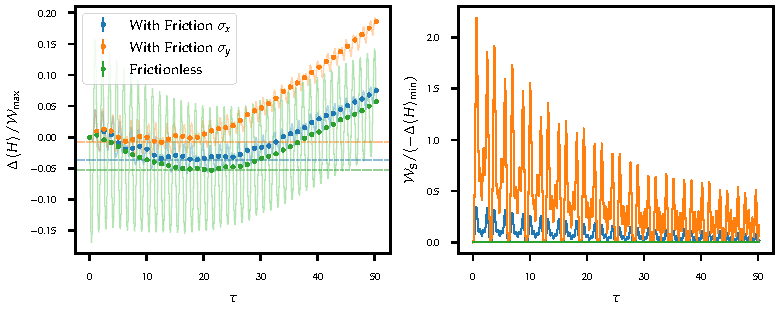
\includegraphics{figs/one_bath_mod/quantum_friction}
  \caption{\label{fig:quant_frict} Total energy change normalized by
    the maximal ergotropy in the left panel and the ergotropy of the system
    state \(ρ_{\sys}\) normalized by the maximal extracted energy
    (dashed lines in left panel) in the right panel over time. Here
    \(λ=0.1, Δ=5, T=5\) was chosen. In the ``With Friction'' case
    \(σ_{f}=σ_{x,y}\) and in the ``Frictionless'' case
    \(σ_{f}=σ_{z}\).  The solid dots mark the times when \(H_{\inter}
    = 0\). The horizontal dashed lines mark the minimal
    total energy differences achieved.  For more parameters see
    \cref{tab:plus_friction}.}
\end{figure}

When choosing \(σ_{f}=σ_{y}\) the situation is even worse, because now
the system modulation does not even commute with the interaction. The
extracted energy is smallest and the relative system ergotropy buildup
is maximal.

\subsection{System Modulation}
\label{sec:sys_mod_v_no_sys_mod}
As it turns out, the modulation generically leads to a deterioration
of energy extraction performance for the model
\cref{eq:one_qubit_model_driven} as is demonstrated in
\cref{fig:quant_frict_sys_no_sys}. Again, the ``friction'' (system
ergotropy) generated by the system modulation is much greater than
without system modulation. However, it is questionable whether this is
the only reason for the performance advantage of the case without
system modulation. Another factor is, that the system goes in and out
of resonance with the bath and therefore hampers energy
extraction.
\begin{figure}[h]
  \centering
  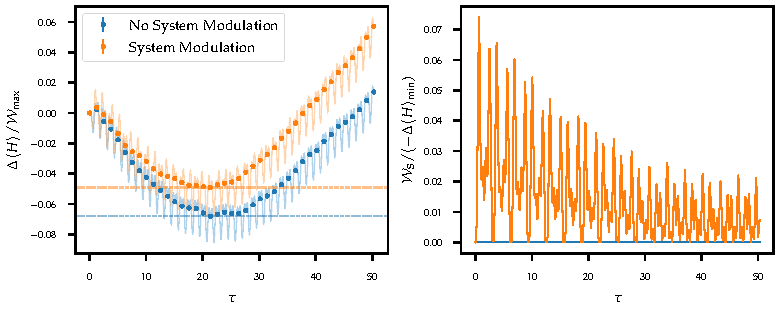
\includegraphics{figs/one_bath_mod/system_vs_no_system}
  \caption{\label{fig:quant_frict_sys_no_sys} Similar to
    \cref{fig:quant_frict}, but for (frictionless) system modulation
    and no system modulation. The parameters were \(λ=0.1, Δ=5, T=5\)
    and further details can be found in \cref{tab:plus_system}.}
\end{figure}

In light of this result we shall continue with \(λ=0\), which
simplifies the situation.

\subsection{Energy Extraction with different Bath Memories}
\label{sec:extr_mem}
To further answer whether a substantial fraction of the maximal
ergotropy can be extracted from a system we have numerically optimized
the coupling strengths of the model \cref{eq:one_qubit_model_driven},
so that over ten modulation periods \(τ_{m} = \frac{2 π}{Δ}\) the
maximal absolute interaction energy is close to a give value (here
\(\ev{H_{\inter}}\approx 0.4\) which constitutes quite a strong
coupling) for various cutoff frequencies \(ω_{c}\).
\begin{figure}[h]
  \centering
  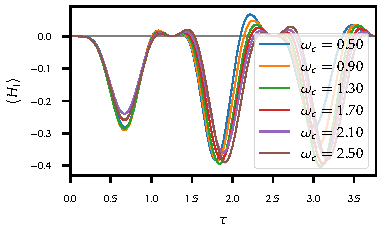
\includegraphics{figs/one_bath_mod/omega_interactions}
  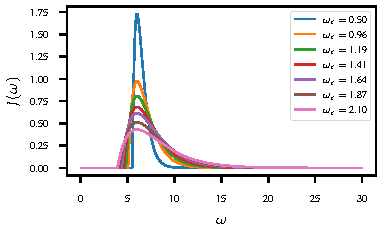
\includegraphics{figs/one_bath_mod/omega_sd}
  \caption{\label{fig:omega_couplings_and_energies} The interaction
    energies and (zero temperature) spectral densities for the
    simulations in this section. Here we used \(λ=0.1, Δ=5, T=5\) and
    the parameters in \cref{tab:plus_omega}.}
\end{figure}

The resulting couplings can be found in
\cref{fig:omega_couplings_and_energies}. They correspond roughly to
demanding \(α_{β}(0)=1.4\), where \(α_{β}\) is the finite temperature
bath correlation function.
\Cref{fig:omega_couplings_and_energies} also shows that for the
simulations with small \(ω_{c}\) the positive parts of the interaction
energy are especially large.

For very weak coupling \(\ev{H_{\inter}}\approx 0.01\)
\cref{fig:omega_couplings_weak} shows that this optimization procedure
yields the normalization of \cref{eq:normohmic}. This is plausible,
because for weaker coupling the initial slip phase upon which
\cref{eq:normohmic} is based stays valid for longer times\fixme{do
  optimization for more periods / slower mod}, albeit that no
modulation was assumed to derive the normalization. For weak coupling,
only the peak value of the spectral density is important and therefore
the peaks must coincide for similar coupling strength.

In \cref{fig:omegas_total} we see the energy extraction behaviour of
the model for various cutoff frequencies.
\begin{figure}[h]
  \centering
  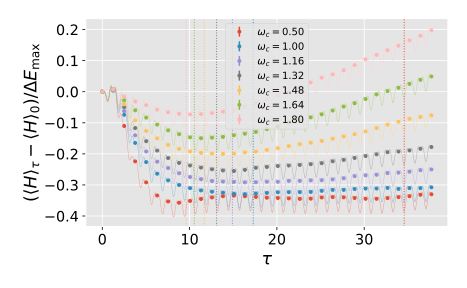
\includegraphics{figs/one_bath_mod/omegas_total}
  \caption{\label{fig:omegas_total} The total energy differences of
    \cref{eq:one_qubit_model_driven} for various \(ω_{c}\). For
    details of the parameters see
    \cref{fig:omega_couplings_and_energies}. The dots mark the times
    when the interaction is turned off.  The dashed lines show the
    position of the where the total energy is minimal.}
\end{figure}
It is clear, that a lower cutoff frequency is advantageous as the
minimal total energy is achieved earlier and is of greater
magnitude. Further, we see that a non-trivial amount of energy is
being extracted relative to ergotropy bound \cref{eq:ergo_mod_model}.

\begin{figure}
  \centering
  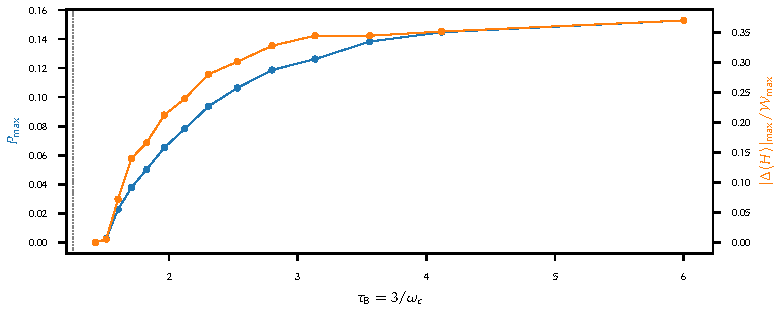
\includegraphics{figs/one_bath_mod/omega_energies_and_powers}
  \caption{\label{fig:omegas_energies_and_powers} One shot power
    (blue) and maximal extracted energy (orange) as a function of
    the bath memory. The grey vertical line marks one
    modulation period.}
\end{figure}
In \cref{fig:omegas_energies_and_powers} we can see that longer
bath\fixme{looks like ``phase transition'' but really isn't} memories,
defined as the time point at which \(α(τ_{\bath}) = α(0)/10\), lead to
both increased energy extraction and increased one shot power. The one
shot power is defined as
\begin{equation}
  \label{eq:one_shot_power}
  P_{\max}=\max_{n\in\NN}\frac{\abs{Δ\ev{H}_{n τ_{m}}}}{n τ_{m}},
\end{equation}
where \(Δ\ev{H}_{τ}= \ev{H}_{τ} - \ev{H}_{0}\).  The concrete shape of
the curve \cref{fig:omegas_energies_and_powers} is hard to discuss
because of the nontrivial shape and magnitude of the spectral
densities. However, the abrupt transition to zero for short memories
is due to the requirement that power and extracted energy have to be
finite, and the stroboscopic time view induced by the requirement that
the interaction energy should be zero.

In conclusion we can say that in the cases studied here we can extract
a finite amount of energy from the system as soon as the bath memory
is somewhat longer than the modulation period. This statement depends
on the definition of the memory time \(τ_{\bath}\) and therefore be
taken as a rule of thumb.

\subsection{Modulation Frequency and Speed Limit}
\label{sec:speedlim}

Another interesting parameter to tune is the modulation frequency
\(Δ\), or equivalently the modulation period time \(τ_{p}=2π/Δ\). In
driven systems, there usually appears a ``quantum speed limit'' that
limits the power output of a driven system at a given coupling
strength. An example is the transition from engine to refrigerator in
a continuously coupled two-bath engine in
\cite{Mukherjee2020Jan}. More generally, this issue is connected to
non-adiabatic changes in the Hamiltonian that can generate non-passive
states \cite{Binder2018}.

Intuitively speaking, slower modulation allows more time for the
system-bath interaction that enables energy extraction from the
initially passive bath state in the first place.

The continuous power is given by
\begin{equation}
  \label{eq:power_for_onequbit}
  P = \ev{\dot{H}_{\inter}} \sim Δ \sin(Δ) \ev{B σ_{x}^{†} + \hc},
\end{equation}
where \(H_{\inter, m} \equiv \ev{B σ_{x}^{†} + \hc}\) constitutes the
unmodulated interaction Hamiltonian. Increasing the frequency \(Δ\)
will increase the amplitude of \cref{eq:power_for_onequbit}. On the
other hand, if the expectation value of \(H_{\inter, m}\) does not
change much, or on a much slower scale than \(τ_{p}\) because of too
fast modulation the \(Δ\sin(Δ)\) factor will cause the expression to
average out to zero (Zeno-like effect, \cite{Kurizki2021Dec}).

Stronger coupling will lead to a greater expectation value of
\(H_{\inter, m}\) and generically to more power.

To assess the behaviour with regard to coupling and modulation speed,
we simulated the model for \(ω_{c}=1\) up to the time \(τ=20\) and
plotted the one shot power \cref{eq:one_shot_power} in a heatmap in
\cref{fig:power_heatmap}. The coupling strength is quantified by the
value of the thermal bath correlation function \(α_{β}\) a time
zero. This balances the shifting of the spectral density for the
different values of \(Δ\).
\begin{figure}[htb]
  \centering
  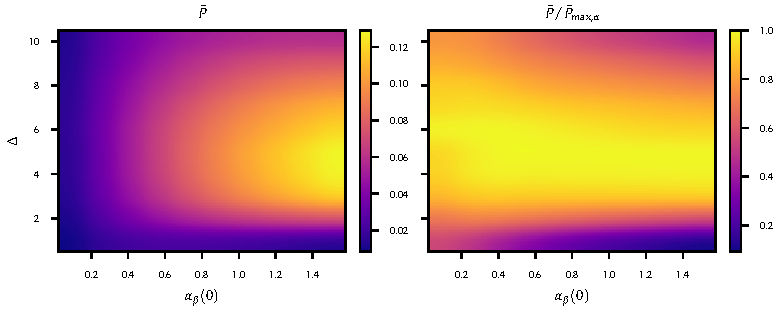
\includegraphics{figs/one_bath_mod/power_heatmap}
  \caption{\label{fig:power_heatmap} Left panel: The one shot power
    \cref{eq:one_shot_power} for the model
    \cref{eq:one_qubit_model_driven} for various modulation
    frequencies \(Δ\) and coupling strengths. The parameters
    \(ω_{c}=1,λ=0.1, T=5\) were used. Right panel: The same, but
    normalized to the maximum power for each \(α_{β}(0)\). In both
    cases \(100\) grid points and Gaussian interpolation have been
    used.}
\end{figure}
\begin{figure}[htb]
  \centering
  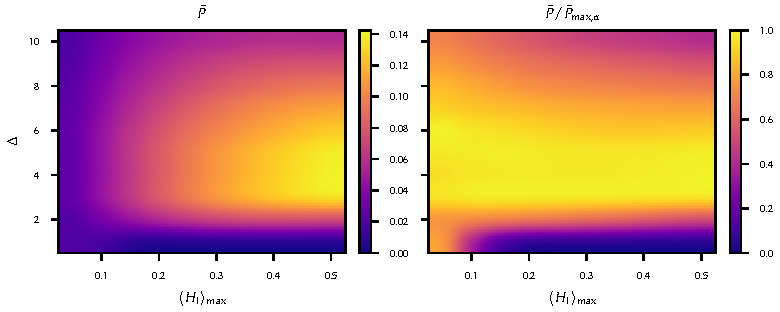
\includegraphics{figs/one_bath_mod/power_en_heatmap}
  \caption{\label{fig:power_heatmap_tuned} Like
    \cref{fig:power_heatmap_tuned} but as function of maximal
    interaction energy as in \cref{sec:extr_mem}.  The parameters of
    the underlying simulations can be found in \cref{tab:plus_mod_en}.}
\end{figure}

We find that the best power output is achieved by stronger
coupling. The dependence on the modulation frequency is more
nuanced. If the power output is normalized by its maximum value for
each \(α_{β}(0)\) it can be seen, that the optimal power output is
achieved at roughly the same modulation frequency. However, with
increasing coupling strength, the system becomes more sensitive to the
modulation frequency, exhibiting a clear maximum. This constitutes the
``speed limit'' discussed above.

Running the simulations with a peak interaction energy target like in
\cref{sec:extr_mem} the results are broadly similar on the level of
detail available to us as can be ascertained from
\cref{fig:power_heatmap_tuned}. For the \(Δ=1\) case the optimization
was generally not very effective in the weaker coupling regime as is
quantified in \cref{fig:interaction_tuning_success}. Therefore this
region should be interpreted with care.

These results have to be taken with a grain of salt however. The grid
resolution of 10 by 10 does not allow us to perceive a shift in the
optimal modulation frequency. Also, the range of interaction strengths
is rather limited.


\begin{figure}[htb]
  \centering
  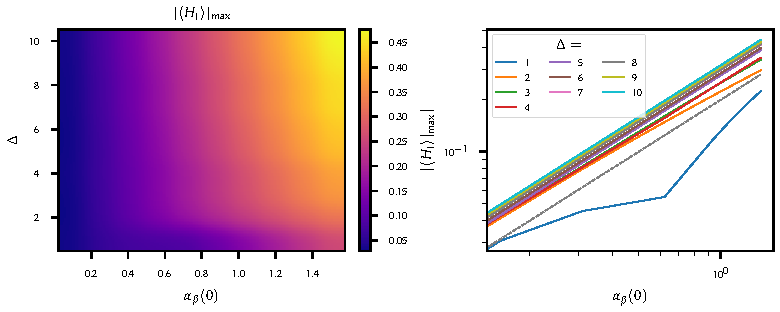
\includegraphics{figs/one_bath_mod/interaction_nontuned}
  \caption{\label{fig:interaction_nontuned} Left panel: Similar to
    \cref{fig:power_heatmap} but showing the maximal absolute
    interaction energies. Right panel: A log-log-plot of the maximal
    interaction energy over the coupling strength. The dashed grey
    line is a linear reference curve.}
\end{figure}

The maximal absolute interaction energies are shown in
\cref{fig:interaction_nontuned} for the non-optimized case of
\cref{fig:power_heatmap} and increase generally with increasing
coupling strength. The dependence on the coupling strength is linear
for modulations with \(Δ\geq 5\) but deviates for slower
modulation. This may be due to the fact, that fewer periods can occur
in the given time frame.

The interaction energy also increases for faster modulation,
especially at greater coupling strengths. Comparing
\cref{fig:interaction_nontuned} with \cref{fig:power_heatmap} we see
that the top right region where the interaction energy is strongest
somewhat coincides with a decrease in power. In this region, the
dependence of the interaction energy on the modulation frequency is
also most pronounced.  The \(Δ=1\) case is an outlier and should
therefore be interpreted with care. It is likely that not enough
cycles have been simulated to judge this case accurately.


Summarizing, we found that the one shot power output for the model
\cref{eq:one_qubit_model_driven} has a complex dependence on the
coupling strength and the modulation frequency. Especially for strong
coupling, the modulation frequency has to be chosen carefully if
maximum energy extraction is desired.

\subsection{Resonance Behaviour of the One Shot Power}
\label{sec:modcoup_reso}

Finally, after having introduced the shift of the spectral density on
a rather vague basis, we would like to give a short example of its
validity.

For this we choose the spectral densities with their peaks slightly
shifted away from \(1+Δ\) to \(1+Δ+δ\) and normalized so that their
peak height is fixed.
\begin{figure}[htb]
  \centering
  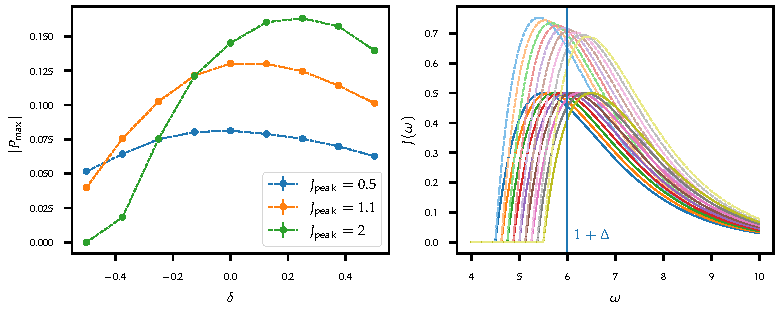
\includegraphics{figs/one_bath_mod/modulation_tuning}
  \caption{\label{fig:modulation_tuning} Left panel: The one shot
    power \cref{eq:one_shot_power} normalized for multiple values of
    the detuning \(δ\) and two peak heights. Right panel: The spectral
    densities for the peak height \(J_{\mathrm{peak}} = 0.5\). The
    dotted lines are the positive frequency parts of the effective
    finite temperature spectral density. The detailed model and
    simulation parameters can be found in \cref{tab:plus_tune}.}
\end{figure}

\Cref{fig:modulation_tuning} shows the result. In all cases, the one
shot power \cref{eq:one_shot_power} as a function of \(δ\) exhibits a
clear maximum which demonstrates the resonance effect.

For the stronger coupling case we find in \cref{fig:modulation_tuning}
that the optimal peak position has moved slightly to the right.
Also the penalty for being off resonant in the negative \(δ\)
direction is much more severe than in the weaker case.

An explanation for the first observation may be, that higher harmonics
like \(1+ 2 Δ\) become important for stronger coupling. Shifting the
spectral density slightly to higher frequencies then optimizes the
coupling.



\section{Quantum Otto Cycle}
\label{sec:otto}
\begin{itemize}
\item multi bath simulations are resource intensive
\item we focus therefore on a simple demonstration of HOPSs usefulness
  in multiple baths
\item an opportunity to test \cref{sec:operational_thermo}
\item also: very popular model and good starting point for future work
\end{itemize}
As a demonstration of a standard thermodynamic cycle that is a popular
model in the literature\footnote{See
  \cite{Wiedmann2021Jun,Karimi2016Nov,Binder2018}.}
is a cyclic quantum heat engine that inspired by the Otto
cycle. Similar to expansion and compression of an ideal gas, we
modulate the level spacing of our working medium. This model servers
as a good demonstration of HOPS' capabilities in terms of being a
method that can treat various bath correlation functions and arbitrary
modulations.

Here, we consider a spin boson model much like the one in
\cref{sec:singlemod} but with two baths
\begin{equation}
  \label{eq:otto_model}
  H = \frac{1+f(t)}{2} (σ_z+1) +
   ∑_{i\in\{h, c\}}\bqty{h_{i}(t) ∑_λ\frac{1}{2}\qty(g_{λ,i} σ_x^† a_{λ,i} + g_{λ,i}^\ast
  σ_x a_{λ,i}^†) + ∑_λ ω_{λ,i} a_{λ,i}^\dag a_{λ,i}.}
\end{equation}

The modulations \(f\) and \(h_{i}\) are periodic and constructed out
of smoothstep\footnote{See \cref{sec:smoothstep}.} functions. Rather
than giving the precise formulas, we instead plot all the modulations
over one period in \cref{fig:ottomod}.
\begin{figure}[htp]
  \centering
  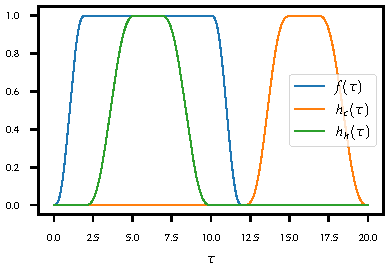
\includegraphics{figs/otto/modulation}
  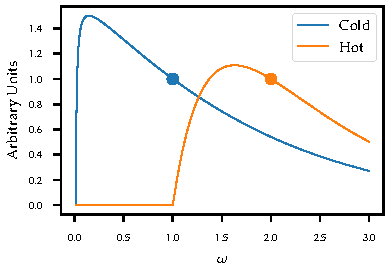
\includegraphics{figs/otto/spectral_densities}
  \caption{\label{fig:ottomod} Left panel: One period of the modulation functions
    in \cref{eq:otto_model}. Right panel: The spectral densities of
    the hot and cold baths. The dots mark the level spacing of the
    system Hamiltonian in the cold and hot phase.}
\end{figure}

First, the energy gap is widened from one to two (widening
stroke). After this, the system is coupled to a hot bath to ``charge''
for some time and decoupled before the energy gap is being compressed
from two to one again (shrinking stroke). Finally, the qubit is being
``reset'' by shedding energy into a low temperature bath.

The effective finite\fixme{explain that?} temperature spectral
densities with \(ω_{c}=1\) have been shifted, such that their value is
maximal for a given temperature at the frequency of the system in its
compressed (cold) or expanded (hot) state. Their magnitudes have been
chosen so that their values at these points are the same as can be
seen in \cref{fig:ottomod}.

We initialize the system in the \(H_{\sys}\ket{0}=0\) state.  For the
demonstration we chose \(T_{c}=1\) and \(T_{h}=20\) so that both
temperatures are finite but not so high that an unreasonable number of
samples is required for convergence. The interaction strength has been
chosen to be relatively weak for the same reason and to be closer to
the known weak coupling realm.

In comparison to the system time scale, the modulation cycle is rather
slow. On the other hand, the time scales on which \(f\) and \(h_{i}\)
change are rather short.

\begin{figure}[htp]
  \centering
  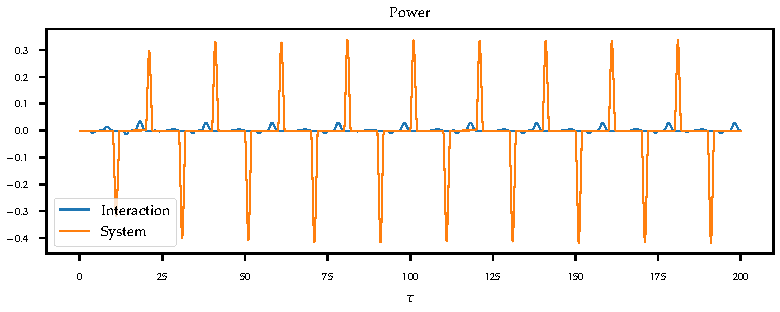
\includegraphics{figs/otto/power}
  \caption{\label{fig:ottopower} The power due to the system and the
    bath modulation of the Otto cycle model \cref{eq:otto_model}. The
    total power is
    \(\ev{\dot{H}} = \ev{\dot{H}_{\sys}} + \ev{\dot{H}_{\inter}}\). }
\end{figure}
\Cref{fig:ottopower} shows the power due to the modulation of the
system and the interaction Hamiltonians. The main contribution to the
power is the system modulation. The shrinking stroke produces negative
(usable) power and the widening produces positive power that has to be
provided externally. More importantly however, we find that also the
modulation of the interaction, i.e. the coupling and decoupling
produce predominantly positive power that has to be put in. In a weak
coupling scheme, this contribution can be neglected. Not so however in
the generic case presented here.

The mean power output of this cycle is
\(\bar{P}=0.002468\pm 0.000021\) with an efficiency of \(η=29\%\),
where the efficiency is defined as in \cref{eq:efficiency_definition}.

Neglecting the energy change due to the coupling
modulation we find instead \(\bar{P}=0.004337\pm 0.000018\) and
\(η=52\%\).  This efficiency is, maybe coincidentally, close to the
efficiency given in \cite{Geva1992Feb} for the quantum Otto cycle
under equilibrium conditions. In any case we are far from the Carnot
efficiency for the given temperatures \(η_{c}=95\%\), as we are not in
the adiabatic regime.

\begin{figure}[htp]
  \centering
  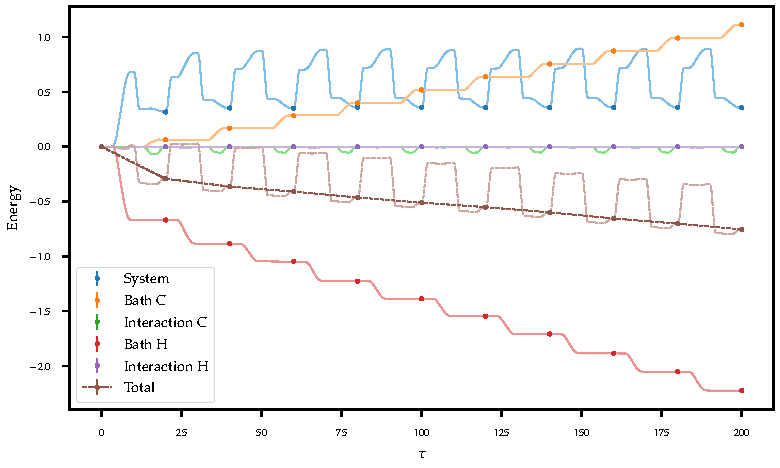
\includegraphics{figs/otto/energy_strobe}
  \caption{\label{fig:ottoenergy} The system, bath and interaction
    energies as well as the total energies of the model
    \cref{eq:otto_model}. The dots mark the times where one cycle is
    completed.}
\end{figure}

In \cref{fig:ottoenergy} we show the full energy dynamics. The
interaction energy for the coupling to the hot bath is almost
negligible, while the interaction with the cold bath is stronger. The
system energy change due to the both is of similar magnitude however.
A periodic steady state is reached after roughly two cycles. In this
steady state, the system and interaction related quantities are
constant in the stroboscopic view (the dots in \cref{fig:ottoenergy}),
while the total energy and the bath energies depend linearly on
time. We do not see no oscillations in the bath energy which would
indicate the more complicated energy transfer behaviour we found in
\cref{sec:one_bath_cutoff}, signifying that we are working in a rather
``tame'' regime as intended.

The Gibbs like inequality \cref{eq:secondlaw_cyclic} derived in
\cref{sec:operational_thermo} can also be verified in this case.
We find
\begin{equation}
  \label{eq:secondlaw_otto_actual}
  ∑_iβ_i ΔE_{\bath^i}^\cyc = 0.1096\pm 0.0008 ≥ 0,
\end{equation}
which does satisfy the inequality to over 100 standard
deviations. Minimizing this quantity would maximize the efficiency.

With this cycle, little coherence is generated\footnote{See
  \cref{eq:otto_coherences}.} leading so called ``frictionless''
dynamics. See also \cref{eq:otto_bloch} for a plot of the trajectory
of the system density matrix in the bloch sphere.

Because it requires little additional effort, we can briefly explore a
continuously coupled version off this model, where the coupling
modulation is turned of and we have \(h_{1}(τ)=1\). We find in
\cref{fig:ottoenergy_cont} that work extraction is still possible,
albeit at a much lower power \(\bar{P}=0.001670\pm 0.000029\) and
efficiency \(η=5\%\).
\begin{figure}[htp]
  \centering
  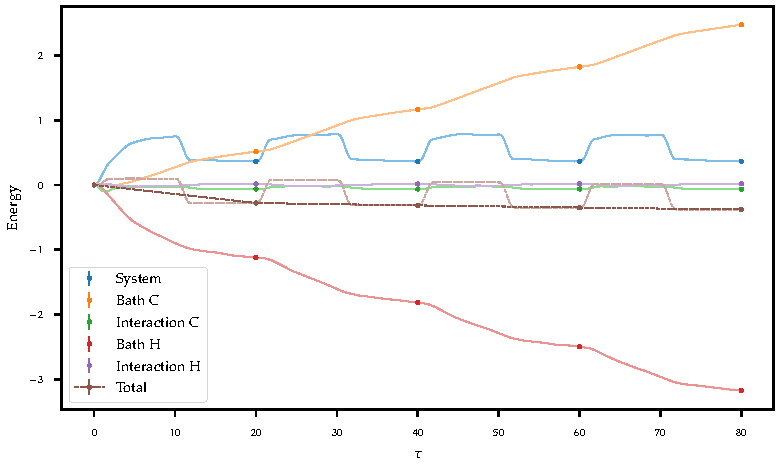
\includegraphics{figs/otto/energy_strobe_continuous}
  \caption{\label{fig:ottoenergy_cont} The system, bath and
    interaction energies as well as the total energies of the model
    \cref{eq:otto_model} for continuously coupled baths. The dots mark
    the times where one cycle is completed. We can observe positive
    energy extraction albeit at a much reduced power
    \(\bar{P}=0.001670\pm 0.000029\) and efficiency \(η=5\%\) compared
    to the modulated case in \cref{fig:ottoenergy}.}
\end{figure}

The finite energy extraction is due to the baths being alternately
resonant and off-resonant. Increasing the amplitude of the system
modulation and consequently the gap between the peaks of the spectral
densities should improve the performance.

The lost efficiency is due to energy flowing ``through'' the system
unused, a behaviour which is promoted by the continous coupling and
reflected in the quantity
\(∑_iβ_i ΔE_{\bath^i}^\cyc = 0.6198\pm 0.0021\) which reflects the
``entropy production'' of the bath that leads to reduced efficiency.

Nevertheless, if the cycle was very fast, the effect of the
(un)coupling of the baths could be so detrimental that the
continuously coupled version of the cycle is superior. See also the
remarks below about \cite{Uzdin2015Sep}.

A worthwhile task for future work would be to verify the results
summarized in \cite{Binder2018} for the Otto cycle. Especially the
optimization for optimal power which leads to the
Novikov–Curzon–Ahlborn efficiency \(η_{ca}=1-\sqrt{T_{c}/T_{h}}\) is
interesting in the case of stronger coupling.

Another interesting cycle to study would be a Carnot-type cycle, where
the modulation of the system and the thermalization with the bath
occur at the same time. Interpolating between Otto and Carnot, as well
as studying the effect of overlapping and shifting strokes is a
fascinating avenue for exploration.

Also more interesting working media, such as a three level system are
of interest. In \cite{Uzdin2015Sep} it is shown, that in certain
regimes quantum coherence can lead to superior power output. In the
same regime different types heat engines are equivalent. Both these
effects have been observed experimentally in \cite{Klatzow2019Mar}. It
would be interesting to see if the slight deviations from theory in
\cite{Klatzow2019Mar} could be explained using HOPS.


\newpage
\section{Anti Zeno Engine}
\label{sec:antizeno}
\begin{itemize}
\item mention concept
\item results not reliable in time for thesis
\item interesting because: non markovian QUANTUM advantage. a bit
  sensational ;P
\end{itemize}

\section{Some Proposals for future Work}
\begin{itemize}
\item a list of ideas and some papers I've came across
\item projects for future theses or papers
\end{itemize}


\begin{itemize}
\item ... list all those nice papers ...
\item the third law
\item look more deeply into the peculiarities in \cref{sec:oneosccomp}
\item verify speculation of energy flow vs non-markvianity: flow
  between two baths though a system
\item three level system -> paper
\item driven spin boson -> paper \cite{Magazzu2018Apr}
\item flows crossing in one point: robust featureu
\item linear regeime of steady state energies -> universal, how far
  does it extend
\item more detailed parameter scans, universality between different models?
\item state changes -> is energy difference = heat + work path
  independent (maybe try different protocols and turn off interaction
  at for beginning and end in an adiabatic way...)
\item compare with results from master equation in \cref{sec:prec_sim}
\item steady state methods, better convergence for long-time
  simulations
\item coupling to single bath: although breach of second law forbidden
  -> cyclical energy transfer for very long bath correlation times
\item filter mode: \cref{sec:shift_sp}
\item otto cycle: sensitivity to timing stronger with stronger coupling?
\end{itemize}
